\documentclass[t,xcolor=dvipsnames]{beamer}

%%%%%%%%%%%%%%%%%%%%%%%% Packages/includes
\usepackage[english]{babel}
%\usepackage[latin1]{inputenc}
\usepackage{times}
\usepackage{pgfpages}
\usepackage{pgfplotstable}
\usepackage{booktabs}
\usepackage{subcaption}
\usepackage{epigraph}
% Antonio's macros
% !TEX root = thesis.tex
\definecolor{accolornotes}{rgb}{0.7,0.3,0.2}
\newcommand{\acnote}[1]{\textcolor{accolornotes}{[{\bf #1}]}}


\definecolor{jscolornotes}{rgb}{0.3,0.7,0.2}
\newcommand{\jsnote}[1]{\textcolor{jscolornotes}{[{\bf #1}]}}


\definecolor{acgray}{rgb}{0.8,0.8,0.8}
\newcommand{\acremove}[1]{\textcolor{acgray}{[{#1}]}}

\definecolor{myred}{rgb}{0.6, 0, 0}
\definecolor{myblue}{rgb}{0.3, 0.1, 0.9}

%\definecolor{acgreen}{rgb}{0.1,0.5,0.1}
%\definecolor{acblue}{rgb}{0.1,0.1,0.5}
%\newcommand{\bl}[1]{\textcolor{acgreen}{#1}}
%\newcommand{\gr}[1]{\textcolor{acblue}{#1}}

\newcommand{\eg}{{\it e.g.}\ }
\newcommand{\ie}{{\it i.e.}\ }
\newcommand{\vs}{{vs.}\ }
\newcommand{\etal}{{et al.}\ }
%\newcommand{\cf}{{\it cf}}

\newcommand{\be}{\begin{equation}}
\newcommand{\ee}{\end{equation}}
\newcommand{\bea}{\begin{eqnarray}}
\newcommand{\eea}{\end{eqnarray}}
\newcommand{\beas}{\begin{eqnarray*}}
\newcommand{\eeas}{\end{eqnarray*}}

\usepackage{tikz}

\newcommand{\circleplus}{ 
  \mathbin{
    \mathchoice
      {\buildcircleplus{\displaystyle}}
      {\buildcircleplus{\textstyle}}
      {\buildcircleplus{\scriptstyle}}
      {\buildcircleplus{\scriptscriptstyle}}
  } 
}

\newcommand\buildcircleplus[1]{%
  \begin{tikzpicture}[baseline=(X.base), inner sep=0, outer sep=0]
    \node[draw,circle] (X)  {$#1+$};
  \end{tikzpicture}%
}


\newcommand{\reflabel}{dummy} % Dummy initial reflabel - use renewcommand at the start of each chapter

%%%
%%% Stuff for vector typesetting  ----------------------------------------
%%%
%%%    e.g. use "\v a" or "\v r" for vectors
%%%
\def\vec#1{\mathchoice{\mbox{\boldmath  $\displaystyle\bf#1$}}
{\mbox{\boldmath  $\textstyle\bf#1$}}
{\mbox{\boldmath  $\scriptstyle\bf#1$}}
{\mbox{\boldmath  $\scriptscriptstyle\bf#1$}}}
\def\v#1{\protect\vec #1}

%%%
%%% Stuff for matrix typesetting  ----------------------------------------
%%%
%%%    e.g. use "\m M" or "\m A" for matrices
%%%
\def\mat#1{\mathchoice{\mbox{\boldmath$\displaystyle\tt#1$}}
{\mbox{\boldmath$\textstyle\tt#1$}}
{\mbox{\boldmath$\scriptstyle\tt#1$}}
{\mbox{\boldmath$\scriptscriptstyle\tt#1$}}}
\def\m#1{\protect\mat #1}

%%%
%%% Stuff for bold maths typesetting  ----------------------------------------
%%%
%%%   e.g. use "\bfmu" for boldface mu symbol
%%%
\def\bfmu{\mbox{\boldmath$\mu$}}
\def\bftau{\mbox{\boldmath$\tau$}}
\def\bftheta{\mbox{\boldmath$\theta$}}
\def\bfdelta{\mbox{\boldmath$\delta$}}
\def\bfphi{\mbox{\boldmath$\phi$}}
\def\bfpsi{\mbox{\boldmath$\psi$}}
\def\bfeta{\mbox{\boldmath$\eta$}}
\def\bfnabla{\mbox{\boldmath$\nabla$}}
\def\bfGamma{\mbox{\boldmath$\Gamma$}}

%%%
%%% Stuff for argmax argmin  ----------------------------------------
%%%
\DeclareMathOperator*{\argmax}{argmax}
\DeclareMathOperator*{\argmin}{argmin}


%%%
%%% Stuff for calligraphic style  ----------------------------------------
%%%
\DeclareMathAlphabet{\mathcal}{OMS}{cmsy}{m}{n}

%% code to highlight maximal/minimal entries in column tables with pgftables
\newcommand{\findmax}[3]{
    \pgfplotstablevertcat{\datatable}{#1}
    \pgfplotstablecreatecol[
    create col/expr={%
    \pgfplotstablerow
    }]{rownumber}\datatable
    \pgfplotstablesort[sort key={#2},sort cmp={float >}]{\sorted}{\datatable}%
    \pgfplotstablegetelem{0}{rownumber}\of{\sorted}%
    \pgfmathtruncatemacro#3{\pgfplotsretval}
    \pgfplotstableclear{\datatable}
}

\newcommand{\findmin}[3]{
    \pgfplotstablevertcat{\datatable}{#1}
    \pgfplotstablecreatecol[
      create col/expr={%
    \pgfplotstablerow
    }]{rownumber}\datatable
    \pgfplotstablesort[sort key={#2},sort cmp={float <}]{\sorted}{\datatable}%
    \pgfplotstablegetelem{0}{rownumber}\of{\sorted}%
    \pgfmathtruncatemacro#3{\pgfplotsretval}
    \pgfplotstableclear{\datatable}
}

\pgfplotstableset{
    highlight col max/.code 2 args={
        \findmax{#1}{#2}{\maxval}
        \edef\setstyles{\noexpand\pgfplotstableset{
                every row \maxval\noexpand\space column #2/.style={
                    postproc cell content/.append style={
                        /pgfplots/table/@cell content/.add={$\noexpand\bf}{$}
                    },
                }
            }
        }\setstyles
    },
    highlight col min/.code 2 args={
        \findmin{#1}{#2}{\minval}
        \edef\setstyles{\noexpand\pgfplotstableset{
                every row \minval\noexpand\space column #2/.style={
                    postproc cell content/.append style={
                        /pgfplots/table/@cell content/.add={$\noexpand\bf}{$}
                    },
                }
            }
        }\setstyles
    },
    highlight row max/.code 2 args={
        \pgfmathtruncatemacro\rowindex{#2-1}
        \pgfplotstabletranspose{\transposed}{#1}
        \findmax{\transposed}{\rowindex}{\maxval}
        \edef\setstyles{\noexpand\pgfplotstableset{
                every row \rowindex\space column \maxval\noexpand/.style={
                    postproc cell content/.append style={
                        /pgfplots/table/@cell content/.add={$\noexpand\bf}{$}
                    },
                }
            }
        }\setstyles
    },
    highlight row min/.code 2 args={
        \pgfmathtruncatemacro\rowindex{#2-1}
        \pgfplotstabletranspose{\transposed}{#1}
        \findmin{\transposed}{\rowindex}{\maxval}
        \edef\setstyles{\noexpand\pgfplotstableset{
                every row \rowindex\space column \maxval\noexpand/.style={
                    postproc cell content/.append style={
                        /pgfplots/table/@cell content/.add={$\noexpand\bf}{$}
                    },
                }
            }
        }\setstyles
    },
}

\makeatletter
\long\def\pgfplotstabletypeset@opt@collectarg[#1]#2{%

    \pgfplotstable@isloadedtable{#2}%
        {\pgfplotstabletypeset@opt@[#1]{#2}}%
        {\pgfplotstabletypesetfile@opt@[#1]{#2}}%
}
\makeatother


\usepackage{tikz}
\usetikzlibrary{arrows,positioning,matrix,scopes,calc,tikzmark,decorations.pathreplacing,shapes,decorations.markings,calc}
\tikzstyle{every picture}+=[remember picture]

%%%%%%%%%%%%%%%%%%%%%%%% Bibliography
\usepackage[backend=bibtex,style=authortitle]{biblatex}
\AtEveryCitekey{\iffootnote{\color{black}\tiny}{\color{black}}}
\addbibresource{../references.bib}

%%%%%%%%%%%%%%%%%%%%%%%% Beamer Mode

%\setbeameroption{hide notes}
%\setbeameroption{show notes}
%\setbeameroption{show notes on second screen=right}


%%%%%%%%%%%%%%%%%%%%%%%% Beamer Options/Settings

\mode<presentation>
{
  \usetheme{default}
  \setbeamercovered{transparent}
}

\AtBeginSection[]{
  \usebackgroundtemplate{
  \tikz[overlay,remember picture] \node[opacity=0.2, at=(current page.center)] {
  \includegraphics[height=\paperheight,width=\paperwidth]{background}};
  }

  \begin{frame}
  \vfill
  \centering
  %\begin{beamercolorbox}[sep=8pt,center,shadow=true,rounded=true]{title}
    \usebeamerfont{title}\insertsectionhead\par%
  %\end{beamercolorbox}
  \vfill
  \end{frame}
  
  \usebackgroundtemplate{}
}

%\setbeamertemplate{note page}[plain]

% Get rid of the annoying symbol list
\beamertemplatenavigationsymbolsempty
% don't show bookmarks on initial view
\hypersetup{pdfpagemode=UseNone}

% Show page number in lower right
\setbeamertemplate{footline}{%
    \raisebox{5pt}{\makebox[\paperwidth]{\hfill\makebox[20pt]{\color{gray}
          \scriptsize\insertframenumber}}}\hspace*{5pt}}


\addtobeamertemplate{frametitle}{}{%
    \begin{tikzpicture}[remember picture,overlay]
    \node[anchor=north east,yshift=2pt] at (current page.north east) {
\includegraphics[height=1em]{uc-cmyk}};
    \end{tikzpicture}}

\definecolor{filtercolor}{RGB}{255,230,153}
\definecolor{filtershade}{RGB}{205,185,123}
\definecolor{fmcolor}{RGB}{231,230,230}
\definecolor{fmshade}{RGB}{186,185,185}

\setbeamercolor{title}{fg=White}
\setbeamercolor{author}{fg=White}
\setbeamercolor{institute}{fg=White}
\setbeamercolor{date}{fg=White}
%\setbeamercolor{section in head/foot}{fg=White}
%\setbeamercolor{author in head/foot}{fg=White}
%\setbeamercolor{date in head/foot}{fg=White}


%%%%%%%%%%%%%%%%%%%%%%%% Title Page Setup
\title[Restricted Connectivity in Deep Neural Networks] % (optional, use only with long paper titles)
{Restricted Connectivity in Deep Neural Networks}
%\subtitle
%{Improving CNN
%Generalization and
%Efficiency}

\author[Yani Ioannou]
{Yani Ioannou}

\institute[University of Cambridge] % (optional, but mostly needed)
{University of Cambridge}

\date{March 21, 2017}

%\pgfdeclareimage[height=0.5cm]{university-logo}{uc-cmyk}
%\logo{\pgfuseimage{university-logo}}

% Delete this, if you do not want the table of contents to pop up at
% the beginning of each subsection:
%\AtBeginSubsection[]
%{
%  \begin{frame}<beamer>{Outline}
%    \tableofcontents[currentsection,currentsubsection]
%  \end{frame}
%}

% If you wish to uncover everything in a step-wise fashion, uncomment
% the following command: 

%\beamerdefaultoverlayspecification{<+->}


\begin{document}

%%%%%%%%%%%%%%%%%%%% TITLE Frame

\usebackgroundtemplate{%             declare it
\tikz[overlay,remember picture] \node[opacity=0.95, at=(current page.center)] {
   \includegraphics[height=\paperheight,width=\paperwidth]{background}};
}

\begin{frame}
  \titlepage
\end{frame}


\usebackgroundtemplate{%             declare it
\tikz[overlay,remember picture] \node[opacity=0.2, at=(current page.center)] {
   \includegraphics[height=\paperheight,width=\paperwidth]{background}};
}

%\begin{frame}{Outline}
%  \tableofcontents
  % You might wish to add the option [pausesections]
%\end{frame}


% - Exactly two or three sections (other than the summary).
% - At *most* three subsections per section.
% - Talk about 30s to 2min per frame. So there should be between about
%   15 and 30 frames, all told.

\section{Research Overview}

\subsection{PhD Research}

\begin{frame}{First Author Publications during PhD}
\begin{itemize}
    \item Decision Forests, Convolutional Networks and the Models in-Between.\\{\footnotesize Y.\ Ioannou, D.\ Robertson, D.\ Zikic, P.\ Kontschieder, J.\ Shotton, M.\ Brown, A.\ Criminisi.\\MSR Technical Report 2015} 
    \item Training CNNs with Low-Rank Filters for Efficient Image Classification.\\{\footnotesize Y.\ Ioannou, D.\ Robertson, J.\ Shotton, R.\ Cipolla, A.\ Criminisi. \\ICLR 2016}
    \item Deep roots: Improving CNN efficiency with hierarchical filter groups.\\{\footnotesize Y.\ Ioannou, D.\ Robertson, R.\ Cipolla, A.\ Criminisi.\\CVPR 2017}
    
\end{itemize}
\end{frame}

\subsection{Collaborative Research}
\begin{frame}{Collaborative Research @ MSR}
\begin{itemize}
    \item \textbf{Medical Computer Vision}
    \begin{itemize}
        \item Segmentation of brain tumor tissues with convolutional neural networks.\\{\footnotesize D.\ Zikic, Y.\ Ioannou, M.\ Brown, A.\ Criminisi.}\\%\\\textit{MICCAI-BRATS 2014}}
        \item Using CNNs for Malaria Diagnosis.\\{\footnotesize Intellectual Ventures/Gates Foundation}
    \end{itemize}
    \item \textbf{Adversarial Examples}\\Measuring Neural Net Robustness with Constraints.\\{\footnotesize O.\ Bastani, Y.\ Ioannou, L.\ Lampropoulos, D.\ Vytiniotis, A.\ Nori, A.\ Criminisi.}%\\\textit{NIPS 2016}}
    \item \textbf{Neural Network Design}\\Refining Architectures of Deep Convolutional Neural Networks.\\{\footnotesize 
S.\ Shankar, D.\ Robertson, Y.\ Ioannou, A.\ Criminisi, R.\ Cipolla.}%\\\textit{CVPR 2016}}
\end{itemize}
\end{frame}


\section{Motivation}

%%%%%%%%%%%%%%%%%%%%

\begin{frame}{AlexNet Complexity}
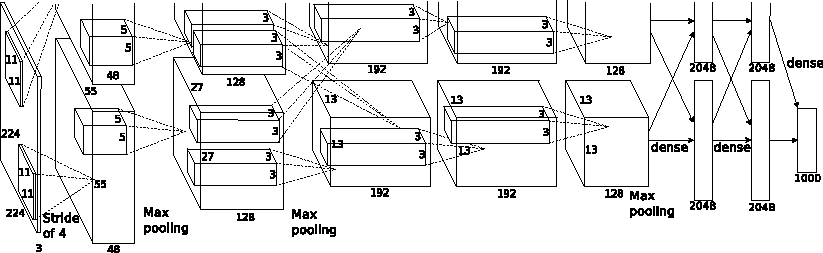
\includegraphics[width=\columnwidth]{alexnet}\footcite{Krizhevsky2012}
\begin{itemize}
\item $\approx$ 61 million parameters %60,965,224
\item $\approx$ 724 million FLOPS (per-sample) % 724,417,384
\item Imagenet has 1.28 million training samples ($227 \times 227 \times 3$) %227×227×3×1281167
\item Images of dimensions  ($227 \times 227 \times 3$) $\approx$ 200 billion pixels % %227×227×3×1281167 = 198,051,763,029
\end{itemize}
\end{frame}
%%%%%%%%%%%%%%%%%%%%


\begin{frame}{Hinton Philosophy}
% http://sms.cam.ac.uk/media/2017973?format=mpeg4&quality=720p
    %\item Standard practice: Create a model of appropriate size for our data and the problem at hand.
    %\item Hinton philosophy on neural network design: Create a massively overparameterized network, and regularize like crazy to prevent overfitting.
    %\item Why is the latter needed in practice?
    %\item ``If you give me any sized dataset, what you ought to do if you want good generalization is get yourself into the small data regime. That is, however big your dataset, you ought to make a much bigger model so that that's small data. So, I think what the brain is doing is making sure that big data is small data and then regularizing the hell out of it, and that's a better thing to do than what statisticians used to think you should do, which is have a small model. And you can think of it as, it's just and efficient way of averaging many, many small models, which is a good way to use argback??, but something a bit more efficient than just doing a normal ensemble. So you should always, if you can, be in the small data regime by having a really big computer. And that's certainly where we live, because we have a limited lifetime so the amount of data we get is limited.''

\begin{quote}
``If you give me any sized dataset, what you ought to do \textbf{if you want good generalization} is get yourself into the small data regime. That is, however big your dataset, you ought to \textbf{make a much bigger model} so that that's small data.''\\

``So, I think what the brain is doing is \ldots \textbf{regularizing the hell} out of it, and that's a better thing to do than what statisticians used to think you should do, which is have a small model.'' \\
\flushright{\normalfont Geoffery Hinton\\\footnote{\url{http://sms.cam.ac.uk/media/2017973}}Cambridge, June 2015}
\end{quote}
\end{frame}

%%%%%%%%%%%%%%%%%%%%

\pgfplotstableread[col sep=comma]{../lrdata/bigpicture.csv}\datatable
\pgfplotstableread[col sep=comma]{../lrdata/bigpicture_ours.csv}\datatableours
\pgfplotstableread[col sep=comma]{../lrdata/bigpicture_aug.csv}\datatableaug
\pgfplotsset{major grid style={dotted,red}}
\pgfplotsset{minor grid style={dotted,red}}

\begin{frame}{}
\resizebox {\textwidth} {!} {
\begin{tikzpicture}
\begin{axis}[
  width=1.2\textwidth,
  height=1.3\textheight,
  axis x line=bottom,
  ylabel=Top-5 Error,
  xlabel=$\log_{10}$(Multiply-Accumulate Operations),
  axis lines=left,
%  enlarge x limits=0.05,
%  enlarge y limits=0.05,
  grid=both,
  ytick={0.00,0.02,...,0.22},
  xmode=log, 
  %ymin=0,ymax=0.2,
  xmin=10e7,xmax=10e13,
  yticklabel={\pgfmathparse{\tick*100}\pgfmathprintnumber{\pgfmathresult}\%},style={
        /pgf/number format/fixed,
        /pgf/number format/precision=1
  },
  legend style={at={(0.99,0.99)},anchor=north east},
]
%\addplot[mark=*,mark options={fill=green!70!black},nodes near coords,only marks,
%   point meta=explicit symbolic,
%   every node near coord/.append style={xshift=0.01em, anchor=west, font=\tiny},
%] table[meta=Network,x=Multiply-Acc.,y expr={1 - \thisrow{Top-5 Acc.} }]{\datatableours};
\addplot[mark=*,mark options={fill=blue},nodes near coords,only marks,
   point meta=explicit symbolic,
   every node near coord/.append style={xshift=0.01em, anchor=west, font=\tiny},
] table[meta=Network,x=Multiply-Acc.,y expr={1 - \thisrow{Top-5 Acc.} }]{\datatable};
\addplot[mark=square*,mark options={fill=red},nodes near coords,only marks,
   point meta=explicit symbolic,
   every node near coord/.append style={xshift=0.01em, anchor=west, font=\tiny},
] table[meta=Network,x=Test Multiply-Acc.,y expr={1 - \thisrow{Top-5 Acc.} }]{\datatableaug};
\legend{Crop \& Mirror Aug., Extra Augmentation}
\end{axis}
\end{tikzpicture}
}
\end{frame}

%%%%%%%%%%%%%%%%%%%%
\begin{frame}{The Problem}
% http://sms.cam.ac.uk/media/2017973?format=mpeg4&quality=720p
\begin{itemize}
%    \item Create a massively over-parameterized network, and ``regularize like hell'' to prevent over-fitting.
%    \item This seems to work well in practice for increasing generalization in networks such as VGG, and MSRA
    \item Creating a massively over-parameterized network, has consequences
    \item Training time: Translates into 2-3 weeks of training on 8 GPUs! (ResNet 200)
    \item Forward pass (ResNet 50): 12 ms GPU, 621 ms CPU
    \item Forward pass (GoogLeNet): 4.4 ms GPU, 300 ms CPU
\end{itemize}
\vfill
But what about the practicalities of using deep learning:
\begin{itemize}
    \item on embedded devices
    \item realtime applications
    \item backed by distributed/cloud computing
\end{itemize}
\end{frame}

%%%%%%%%%%%%%%%%%%%%
\begin{frame}{Alternative Philosophy}
\begin{columns}[onlytextwidth,T]
\begin{column}{0.65\textwidth}
\begin{itemize}
    \item Deep networks need many more parameters than data points because they aren't just learning to model data, but also learning what \emph{\color{blue}not} to learn. 
    %\item At each level in a CNN, the transformed data exists both as weights and spatial/channel information.
    %\begin{itemize}
    %    \item Isn't this what regularization is for? Yes, but it's more like using a sledgehammer on a small nail.
    %\end{itemize}
    % Sort of like regularization, but regularization is like using a sledge hammer on a nail, it affect a lot more than what you want
    \item Idea: Why don't we help the network, through structural priors, not to learn things it doesn't need to?
    %\item Let's separate learning into two distinct functions:
    %\begin{itemize}
    %    \item Learning weights such that a filter responds to a stimulus
    %    \item Learning what to ignore
    %\end{itemize}
    %\item But is that deep? Yann LeCun says not to hand design, learn end-to-end!
\end{itemize}
\end{column}
\begin{column}{0.34\textwidth}
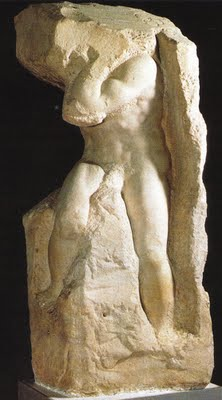
\includegraphics[width=\textwidth]{statue}\\
\tiny \flushright 
The Atlas Slave\\(Accademia, Florence)
\end{column}
\end{columns}
\end{frame}

\section{Structural Priors}

%%%%%%%%%%%%%%%%%

\begin{frame}{Typical Convolutional Layer}
\begin{figure}
   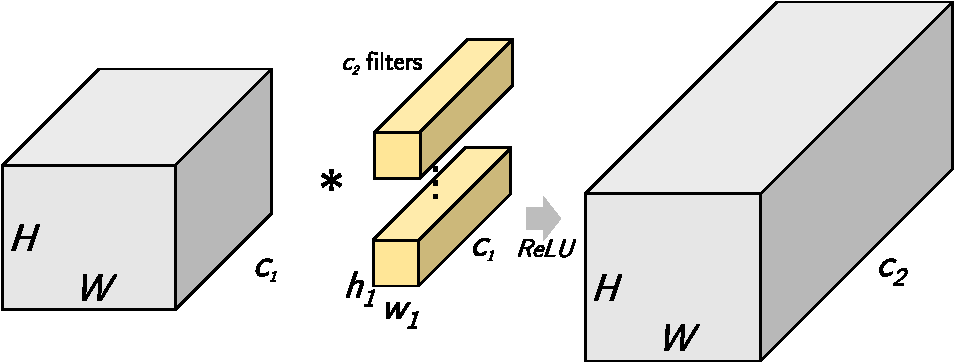
\includegraphics[width=0.9\textwidth, page=1]{../Figs/PDF/groupfig}
%   \caption{A full rank convolutional layer.}
\end{figure}
\begin{figure}

   \resizebox {0.5\textwidth} {!} {
   \begin{tikzpicture}[
       decoration={
          markings,
          mark=at position 1 with {\arrow[scale=2,gray]{latex}};
        }]
        % draw featuremap
        \pgfmathsetmacro{\cubex}{2}
        \pgfmathsetmacro{\cubey}{2}
        \pgfmathsetmacro{\cubez}{1.5}
        \draw[black,fill=fmcolor] (0,0,0) -- ++(-\cubex,0,0) -- ++(0,-\cubey,0) -- ++(\cubex,0,0) -- cycle;
        \draw[black,fill=fmshade] (0,0,0) -- ++(0,0,-\cubez) -- ++(0,-\cubey,0) -- ++(0,0,\cubez) -- cycle;
        \draw[black,fill=fmcolor] (0,0,0) -- ++(-\cubex,0,0) -- ++(0,0,-\cubez) -- ++(\cubex,0,0) -- cycle;
        \draw (-0.7, -2.5) node {image/feature map};
        
        \draw (1, -0.7) node {\LARGE$*$};
        
        % draw filter
        \pgfmathsetmacro{\cubex}{0.3}
        \pgfmathsetmacro{\cubey}{0.3}
        \pgfmathsetmacro{\cubez}{1.5}
        \draw[black,fill=filtercolor] (2,-0.7,0) -- ++(-\cubex,0,0) -- ++(0,-\cubey,0) -- ++(\cubex,0,0) -- cycle;
        \draw[black,fill=filtershade] (2,-0.7,0) -- ++(0,0,-\cubez) -- ++(0,-\cubey,0) -- ++(0,0,\cubez) -- cycle;
        \draw[black,fill=filtercolor] (2,-0.7,0) -- ++(-\cubex,0,0) -- ++(0,0,-\cubez) -- ++(\cubex,0,0) -- cycle;
        \draw (2.2, -2.5) node {filter};
            
        % draw output featuremap
        \pgfmathsetmacro{\cubex}{2}
        \pgfmathsetmacro{\cubey}{2}
        \pgfmathsetmacro{\cubez}{0.1}
        \draw[black,fill=fmcolor] (6,0,-0.75) -- ++(-\cubex,0,0) -- ++(0,-\cubey,0) -- ++(\cubex,0,0) -- cycle;
        \draw[black,fill=fmshade] (6,0,-0.75) -- ++(0,0,-\cubez) -- ++(0,-\cubey,0) -- ++(0,0,\cubez) -- cycle;
        \draw[black,fill=fmcolor] (6,0,-0.75) -- ++(-\cubex,0,0) -- ++(0,0,-\cubez) -- ++(\cubex,0,0) -- cycle;
        \draw (-0.7, -2.5) node {image/feature map};
        
        \draw[gray,postaction={decorate}] (2.7,-0.7) -- (3.8, -0.7);
        
        \draw (5.2, -2.5) node {output featuremap};
    \end{tikzpicture}
    }
\end{figure}
    \note[item]{We show here a typical convolutional layer.}
    \note[item]{Yellow blocks are filters.}
    \note[item]{Grey blocks are images or feature maps.}
\end{frame}

%%%%%%%%%%%%%%%%%%%%
\begin{frame}{Sparsity of Convolution}
\begin{figure}
    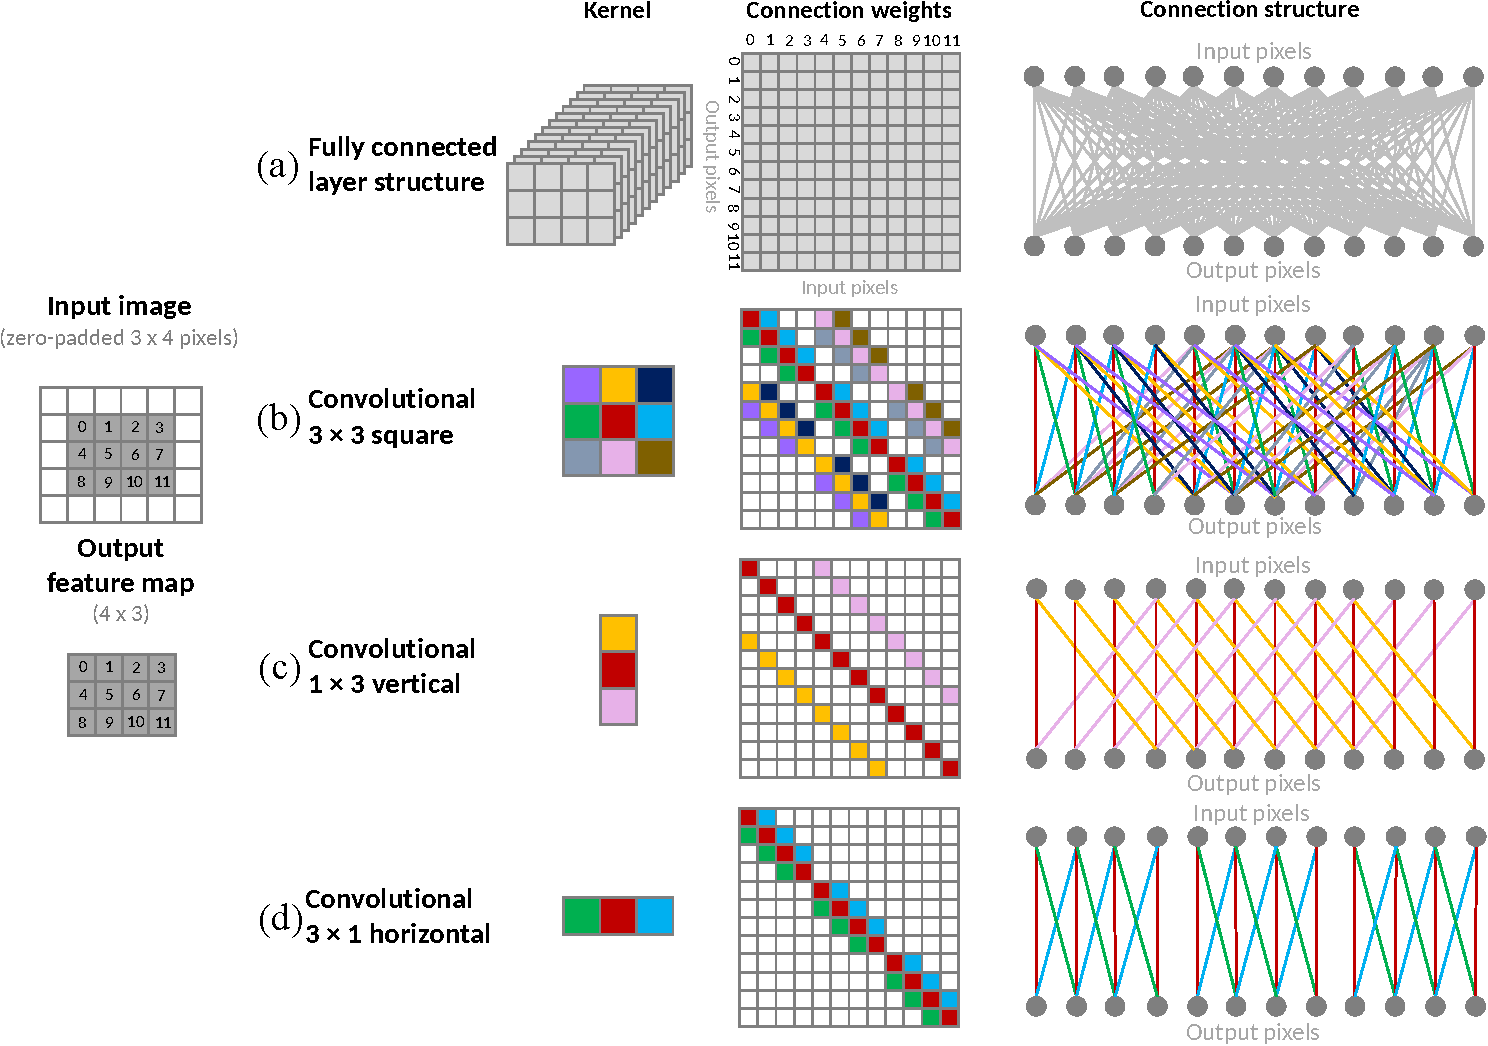
\includegraphics[width=\textwidth]{../Figs/PDF/sparseconn3}
\end{figure}
\end{frame}
%%%%%%%%%%%%%%%%%%%%
\begin{frame}{Why are CNNs uniformly structured?}
\begin{quote}
``The marvelous powers of the brain emerge not from any single, uniformly structured
connectionist network but from highly evolved arrangements of smaller, specialized
networks which are interconnected in very specific ways.''\\
\flushright{\normalfont Marvin Minsky\\Perceptrons (1988 edition)}
\end{quote}
\begin{itemize}
    \item Deep networks are largely monolithic (uniformly connected), with few exceptions
    \item Why don't we try to structure our networks closer to the specialized components required for learning images?
\end{itemize}
\end{frame}

%%%%%%%%%%%%%%%%%%%%
\subsection{Spatial Structural Priors}

\usebackgroundtemplate{%             declare it
\tikz[overlay,remember picture] \node[opacity=0.7, at=(current page.center), yshift=-7cm] {
   \setlength{\fboxsep}{0pt}\fbox{
   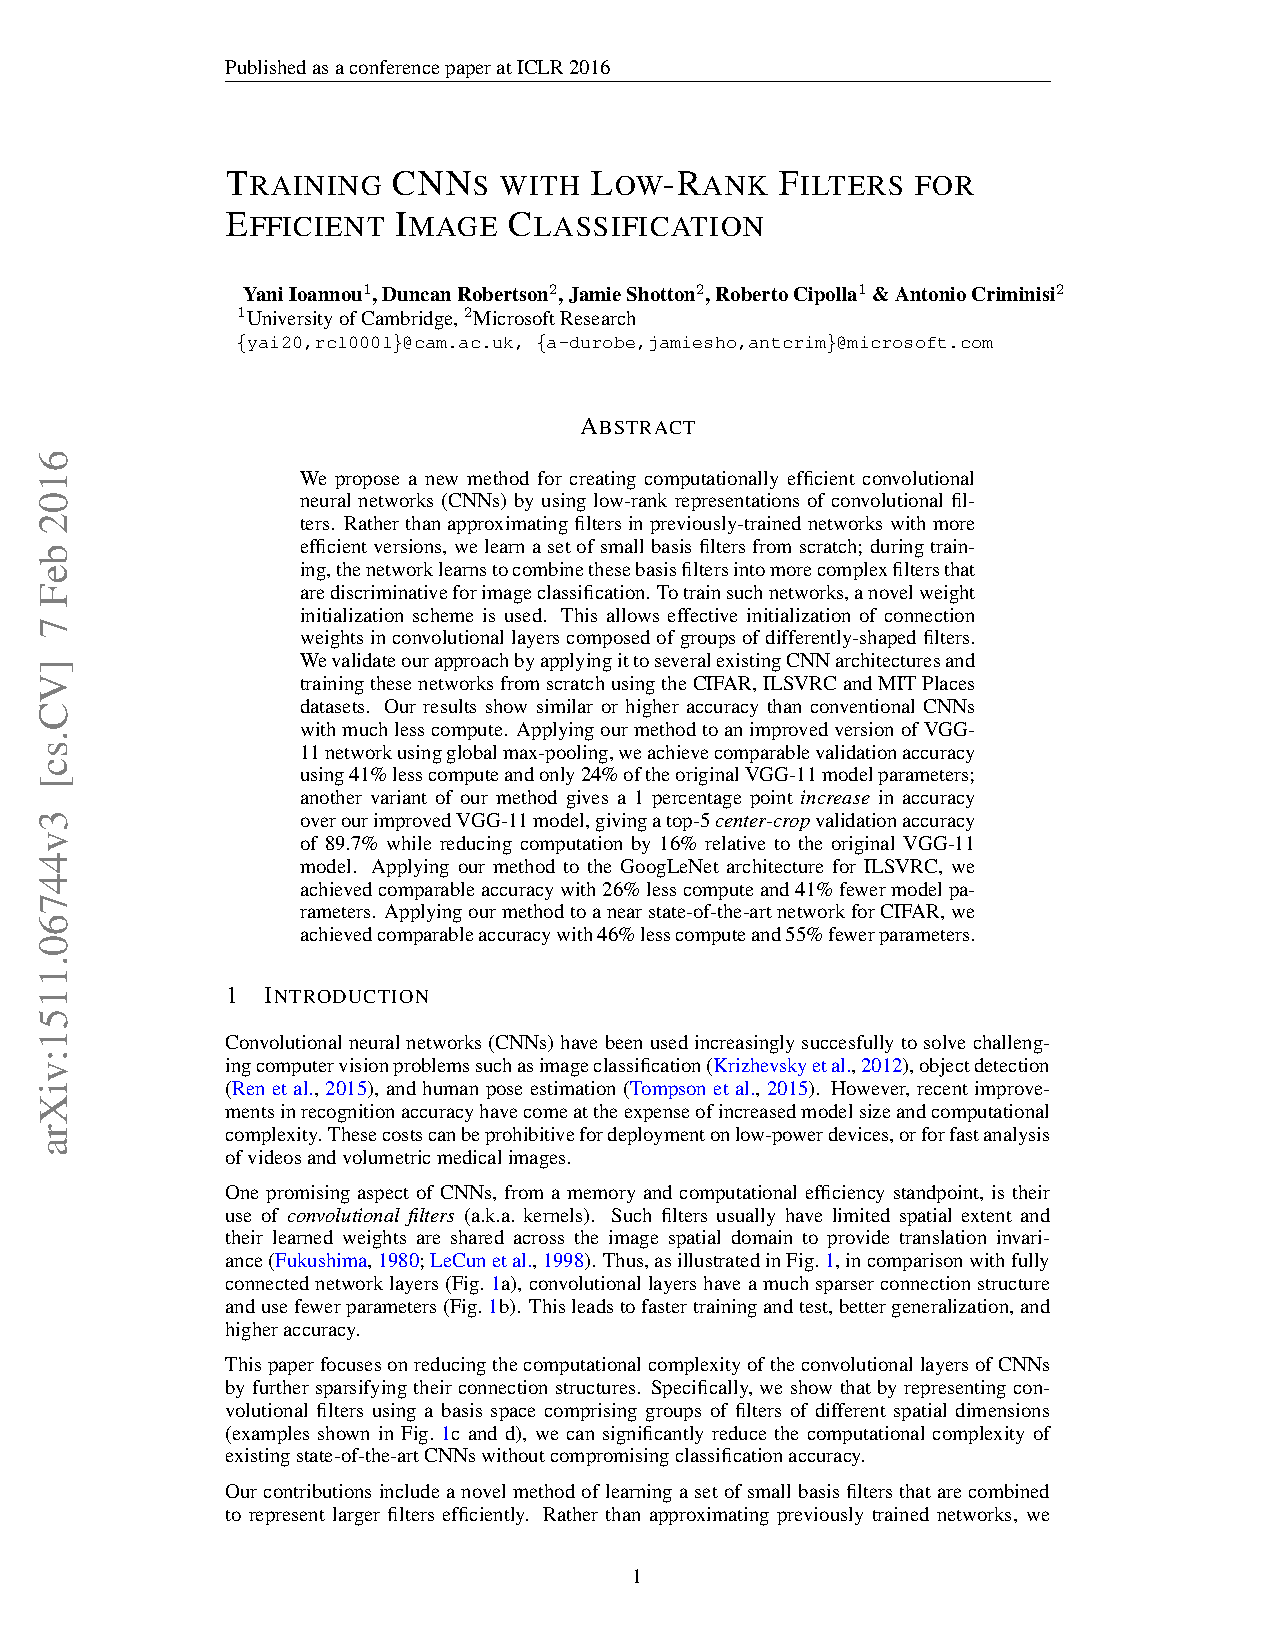
\includegraphics[width=0.9\paperwidth,page=1]{lrpaper.pdf}
   }
   };
}

\begin{frame}
\vfill
\centering
%\begin{beamercolorbox}[sep=8pt,center,shadow=true,rounded=true]{title}
\usebeamerfont{title}Spatial Structural Priors\par%
%\end{beamercolorbox}
\vfill
%Chiseling out the spatial
\end{frame}

\usebackgroundtemplate{}

%%%%%%%%%%%%%%%%%%%%
\begin{frame}{Proposed Method}{Learning a basis for filters.}
\begin{figure}
   \includegraphics[width=\textwidth, page=4]{../Figs/PDF/sparsification}
\end{figure}
\begin{itemize}
    \item A learned basis of vertical/horizontal rectangular filters and square filters!
    \item Shape of learned filters is a full $w \times h \times c$.
    \item But what can be effectively learned is limited by the number and complexity of the components.
\end{itemize}
\end{frame}

%%%%%%%%%%%%%%%%%%%

\begin{frame}{Imagenet Results}

%Applying our method to an improved version of VGG-11 network using global max-pooling, we achieve comparable validation accuracy using 41% less compute and only 24% of the original VGG-11 model parameters; another variant of our method gives a 1 percentage point increase in accuracy over our improved VGG-11 model, giving a top-5 center-crop validation accuracy of 89.7% while reducing computation by 16% relative to the original VGG-11 model. Applying our method to the GoogLeNet architecture for ILSVRC, we achieved comparable accuracy with 26% less compute and 41% fewer model parameters.
%Applying our method to a near state-of-the-art network for CIFAR, we achieved comparable accuracy with 46% less compute and 55% fewer parameters. Networks with root modules have similar or higher accuracy than the baseline architectures with much less computation.
\begin{itemize}
    \item VGG-11 (low-rank): \textbf{24\%} smaller, \textbf{41\%} fewer FLOPS
    \item VGG-11 (low-rank/full-rank mix): \textbf{16\%} fewer FLOPS with \textbf{1\% lower error} on ILSRVC val, but 16\% larger.
    \item GoogLeNet: \textbf{41\%} smaller, \textbf{26\%} fewer FLOPS
\end{itemize}
\vfill
Or better results if you tune it on GoogLeNet more\ldots
\end{frame}
%%%%%%%%%%%%%%%%%%%%

\usebackgroundtemplate{
\tikz[overlay,remember picture] \node[opacity=0.5, at=(current page.center), yshift=-1cm] {
\centering
   \setlength{\fboxsep}{0pt}\setlength\fboxrule{0.5pt}\fbox{
   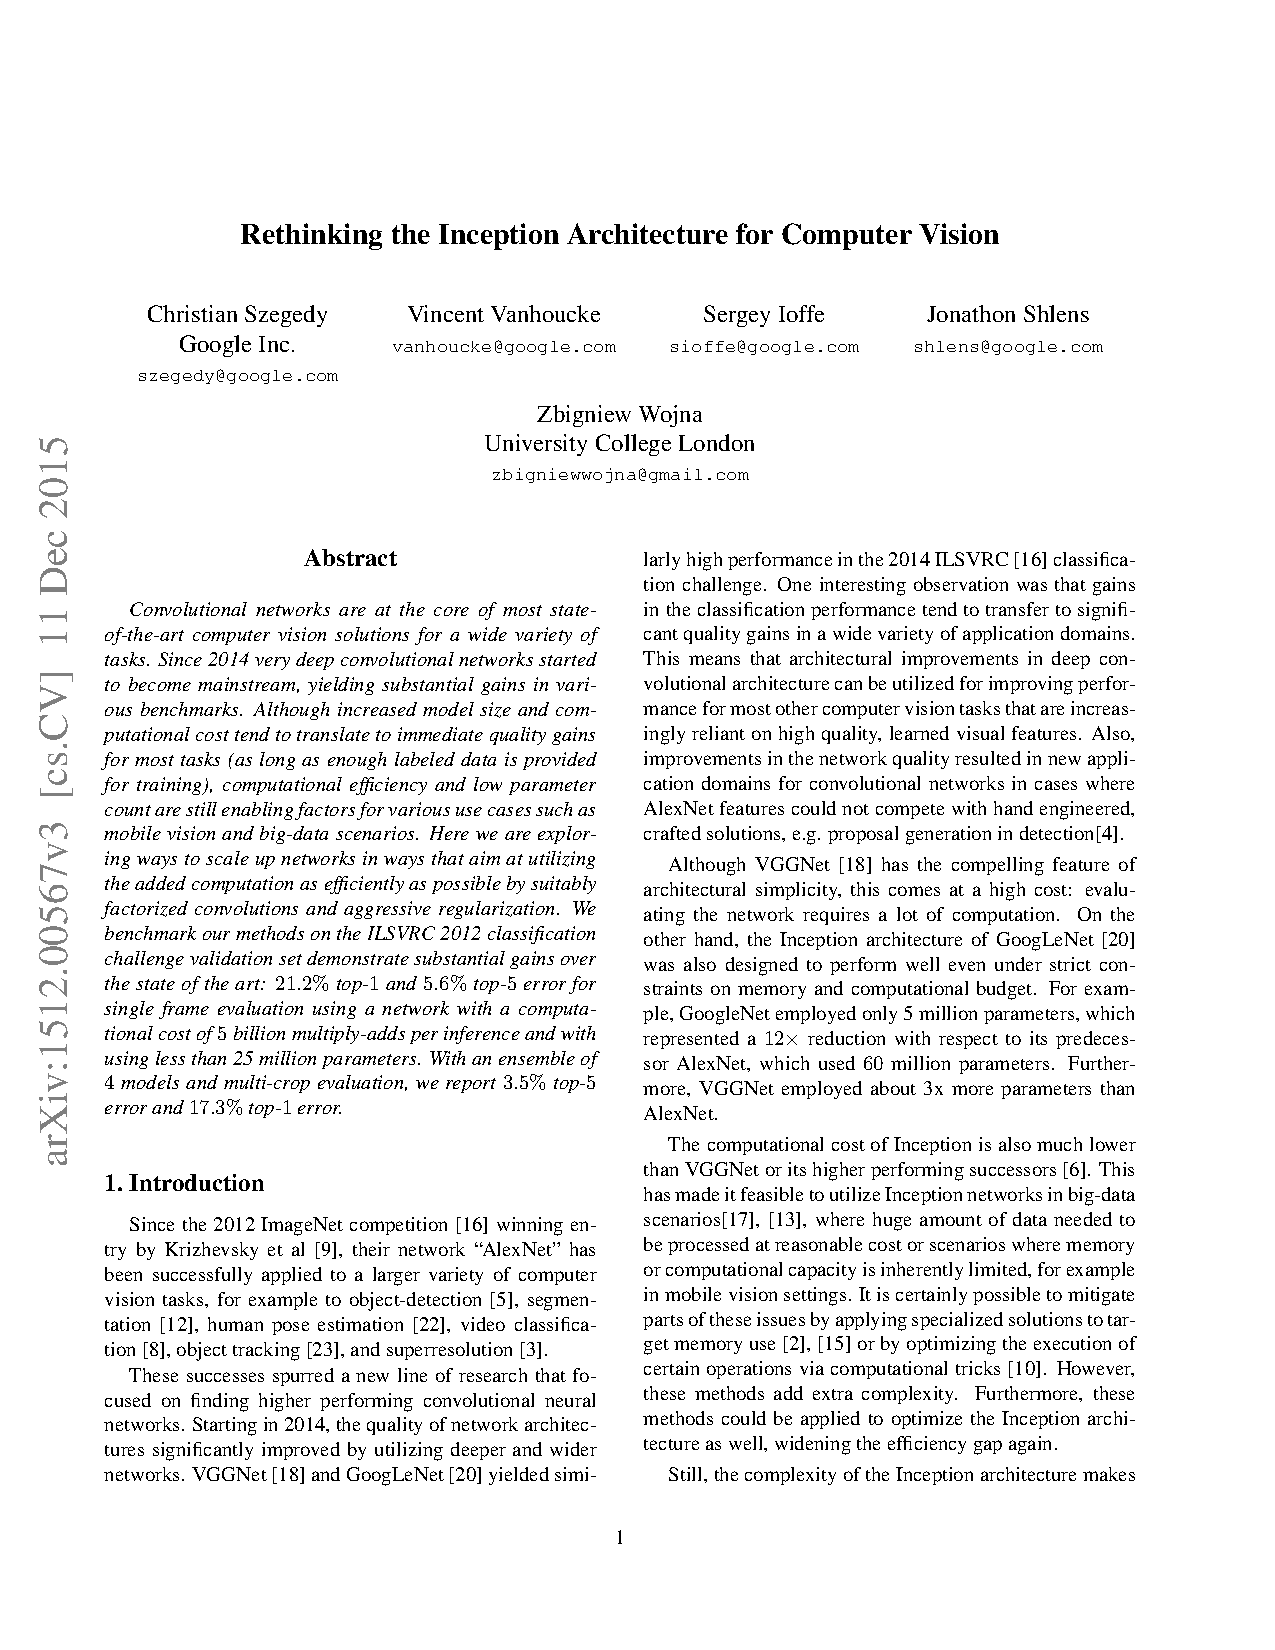
\includegraphics[width=0.9\paperwidth,page=1]{inceptionv3.pdf}
   }
   };
}

\begin{frame}
\vfill
\centering
\colorbox{white}{
\setlength{\fboxsep}{0pt}\fbox{
\begin{minipage}{0.6\paperwidth}
   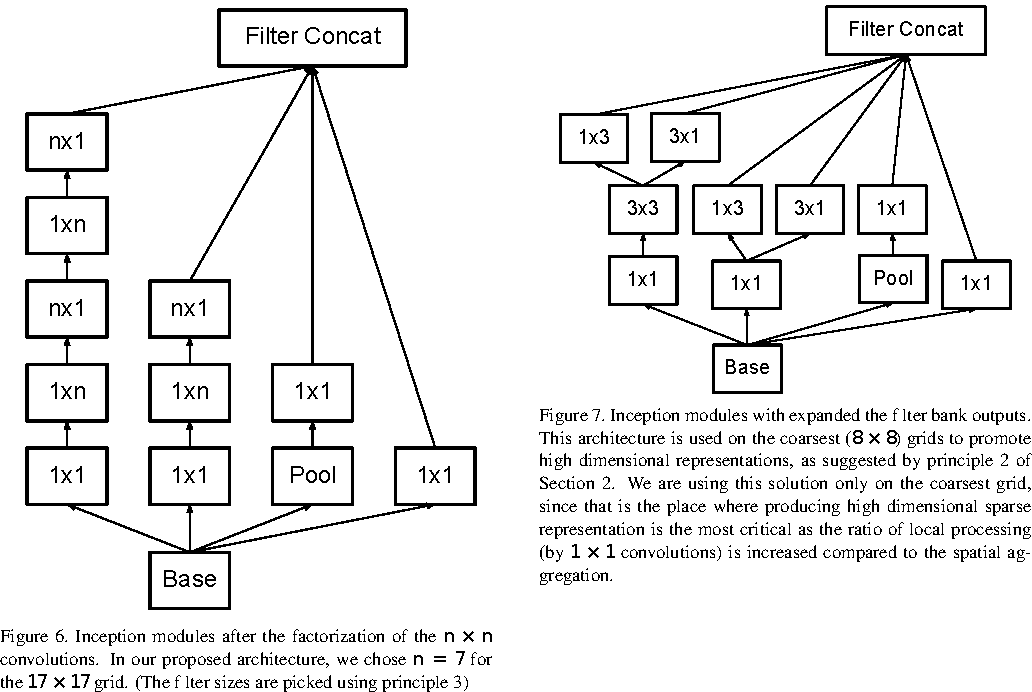
\includegraphics[width=0.6\paperwidth,page=1]{inceptionv3-filterconfig.pdf}
\end{minipage}}}
\end{frame}

\usebackgroundtemplate{}

%%%%%%%%%%%%%%%%%%%%

\subsection{Filter-wise Structural Priors}

\usebackgroundtemplate{%             declare it
\tikz[overlay,remember picture] \node[opacity=0.7, at=(current page.center), yshift=-7cm] {
   \setlength{\fboxsep}{0pt}\fbox{
   \includegraphics[width=0.9\paperwidth,page=1]{deeproots.pdf}
   }
   };
}

\begin{frame}
\vfill
\centering
%\begin{beamercolorbox}[sep=8pt,center,shadow=true,rounded=true]{title}
\usebeamerfont{title}Filter-wise Structural Priors\par%
%\end{beamercolorbox}
\vfill
\end{frame}

\usebackgroundtemplate{}

%%%%%%%%%%%%%%%%%%%%
\begin{frame}{Typical Convolutional Layer}
\begin{figure}
   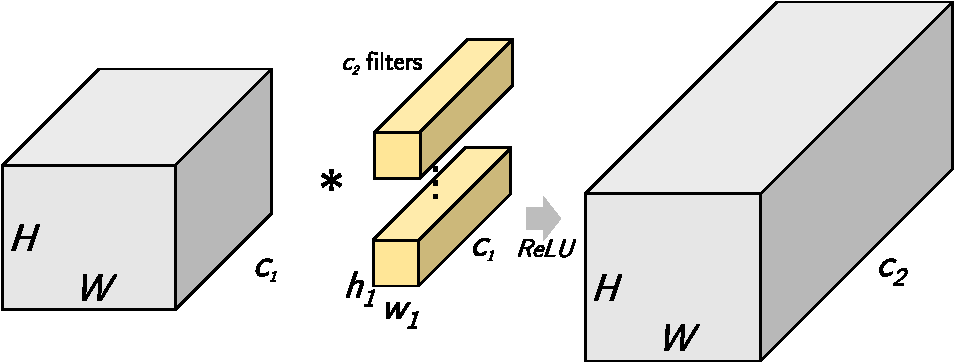
\includegraphics[width=0.9\textwidth, page=1]{../Figs/PDF/groupfig}
%   \caption{A full rank convolutional layer.}
\end{figure}
\begin{figure}

   \resizebox {0.5\textwidth} {!} {
   \begin{tikzpicture}[
       decoration={
          markings,
          mark=at position 1 with {\arrow[scale=2,gray]{latex}};
        }]
        % draw featuremap
        \pgfmathsetmacro{\cubex}{2}
        \pgfmathsetmacro{\cubey}{2}
        \pgfmathsetmacro{\cubez}{1.5}
        \draw[black,fill=fmcolor] (0,0,0) -- ++(-\cubex,0,0) -- ++(0,-\cubey,0) -- ++(\cubex,0,0) -- cycle;
        \draw[black,fill=fmshade] (0,0,0) -- ++(0,0,-\cubez) -- ++(0,-\cubey,0) -- ++(0,0,\cubez) -- cycle;
        \draw[black,fill=fmcolor] (0,0,0) -- ++(-\cubex,0,0) -- ++(0,0,-\cubez) -- ++(\cubex,0,0) -- cycle;
        \draw (-0.7, -2.5) node {image/feature map};
        
        \draw (1, -0.7) node {\LARGE$*$};
        
        % draw filter
        \pgfmathsetmacro{\cubex}{0.3}
        \pgfmathsetmacro{\cubey}{0.3}
        \pgfmathsetmacro{\cubez}{1.5}
        \draw[black,fill=filtercolor] (2,-0.7,0) -- ++(-\cubex,0,0) -- ++(0,-\cubey,0) -- ++(\cubex,0,0) -- cycle;
        \draw[black,fill=filtershade] (2,-0.7,0) -- ++(0,0,-\cubez) -- ++(0,-\cubey,0) -- ++(0,0,\cubez) -- cycle;
        \draw[black,fill=filtercolor] (2,-0.7,0) -- ++(-\cubex,0,0) -- ++(0,0,-\cubez) -- ++(\cubex,0,0) -- cycle;
        \draw (2.2, -2.5) node {filter};
            
        % draw output featuremap
        \pgfmathsetmacro{\cubex}{2}
        \pgfmathsetmacro{\cubey}{2}
        \pgfmathsetmacro{\cubez}{0.1}
        \draw[black,fill=fmcolor] (6,0,-0.75) -- ++(-\cubex,0,0) -- ++(0,-\cubey,0) -- ++(\cubex,0,0) -- cycle;
        \draw[black,fill=fmshade] (6,0,-0.75) -- ++(0,0,-\cubez) -- ++(0,-\cubey,0) -- ++(0,0,\cubez) -- cycle;
        \draw[black,fill=fmcolor] (6,0,-0.75) -- ++(-\cubex,0,0) -- ++(0,0,-\cubez) -- ++(\cubex,0,0) -- cycle;
        \draw (-0.7, -2.5) node {image/feature map};
        
        \draw[gray,postaction={decorate}] (2.7,-0.7) -- (3.8, -0.7);
        
        \draw (5.2, -2.5) node {output featuremap};
    \end{tikzpicture}
    }
\end{figure}
    \note[item]{We show here a typical convolutional layer.}
    \note[item]{Yellow blocks are filters.}
    \note[item]{Grey blocks are images or feature maps.}
\end{frame}

%%%%%%%%%%%%%%%%%%%%

\begin{frame}{Grouped Convolutional Layer}
\begin{figure}
   \includegraphics[width=0.9\textwidth, page=2]{../Figs/PDF/groupfig}
%   \caption{A full rank convolutional layer.}
\end{figure}
\begin{figure}

   \resizebox {0.5\textwidth} {!} {
   \begin{tikzpicture}[
       decoration={
          markings,
          mark=at position 1 with {\arrow[scale=2,gray]{latex}};
        }]
        % draw featuremap
        \pgfmathsetmacro{\cubex}{2}
        \pgfmathsetmacro{\cubey}{2}
        \pgfmathsetmacro{\cubez}{1.5}
        \draw[black,fill=fmcolor] (0,0,0) -- ++(-\cubex,0,0) -- ++(0,-\cubey,0) -- ++(\cubex,0,0) -- cycle;
        \draw[black,fill=fmshade] (0,0,0) -- ++(0,0,-\cubez) -- ++(0,-\cubey,0) -- ++(0,0,\cubez) -- cycle;
        \draw[black,fill=fmcolor] (0,0,0) -- ++(-\cubex,0,0) -- ++(0,0,-\cubez) -- ++(\cubex,0,0) -- cycle;
        \draw (-0.7, -2.5) node {image/feature map};
        
        \draw (1, -0.7) node {\LARGE$*$};
        
        % draw filter
        \pgfmathsetmacro{\cubex}{0.3}
        \pgfmathsetmacro{\cubey}{0.3}
        \pgfmathsetmacro{\cubez}{1.5}
        \draw[black,fill=filtercolor] (2,-0.7,0) -- ++(-\cubex,0,0) -- ++(0,-\cubey,0) -- ++(\cubex,0,0) -- cycle;
        \draw[black,fill=filtershade] (2,-0.7,0) -- ++(0,0,-\cubez) -- ++(0,-\cubey,0) -- ++(0,0,\cubez) -- cycle;
        \draw[black,fill=filtercolor] (2,-0.7,0) -- ++(-\cubex,0,0) -- ++(0,0,-\cubez) -- ++(\cubex,0,0) -- cycle;
        \draw (2.2, -2.5) node {filter};
            
        % draw output featuremap
        \pgfmathsetmacro{\cubex}{2}
        \pgfmathsetmacro{\cubey}{2}
        \pgfmathsetmacro{\cubez}{0.1}
        \draw[black,fill=fmcolor] (6,0,-0.75) -- ++(-\cubex,0,0) -- ++(0,-\cubey,0) -- ++(\cubex,0,0) -- cycle;
        \draw[black,fill=fmshade] (6,0,-0.75) -- ++(0,0,-\cubez) -- ++(0,-\cubey,0) -- ++(0,0,\cubez) -- cycle;
        \draw[black,fill=fmcolor] (6,0,-0.75) -- ++(-\cubex,0,0) -- ++(0,0,-\cubez) -- ++(\cubex,0,0) -- cycle;
        \draw (-0.7, -2.5) node {image/feature map};
        
        \draw[gray,postaction={decorate}] (2.7,-0.7) -- (3.8, -0.7);
        
        \draw (5.2, -2.5) node {output featuremap};
    \end{tikzpicture}
    }
\end{figure}
    \note[item]{We show here a grouped convolutional layer.}
    \note[item]{Yellow blocks are filters.}
    \note[item]{Grey blocks are images or feature maps.}
\end{frame}

%%%%%%%%%%%%%%%%%%%%

%%%%%%%%%%%%%%%%%%%%
\section*{Results}

\newcommand{\covarlabels}[1]{%
\tiny
\vspace{0.75em}
\begin{tikzpicture}[remember picture]
\node [anchor=south west, inner sep=0pt] (c)
    {
        #1
    };
    \path[use as bounding box] (c.south west) rectangle (c.north east);
    \node [anchor=south west, xshift=-0.5em, yshift=-0.5em, rotate=45] at (c.north west) {\footnotesize 0};
    \node [anchor=south east, xshift=\linewidth, yshift=-0.2em] at (c.north west) {\footnotesize 192};
    \node [anchor=south west, xshift=0.25em, yshift=-1.05\linewidth, rotate=90] at (c.north west) {\footnotesize 192};
    \node [anchor=south, xshift=0.5\linewidth] at (c.north west) {\footnotesize\texttt{conv3a}};
    \node [anchor=south, xshift=0.2em, yshift=-0.5\linewidth, rotate=90] at (c.north west) {\footnotesize \texttt{conv2c}};
\end{tikzpicture}%
}

\begin{frame}{Inter-layer Filter Covariance}

\begin{figure}[tb]
\centering
\begin{subfigure}[b]{0.31\linewidth}
\centering
    \covarlabels{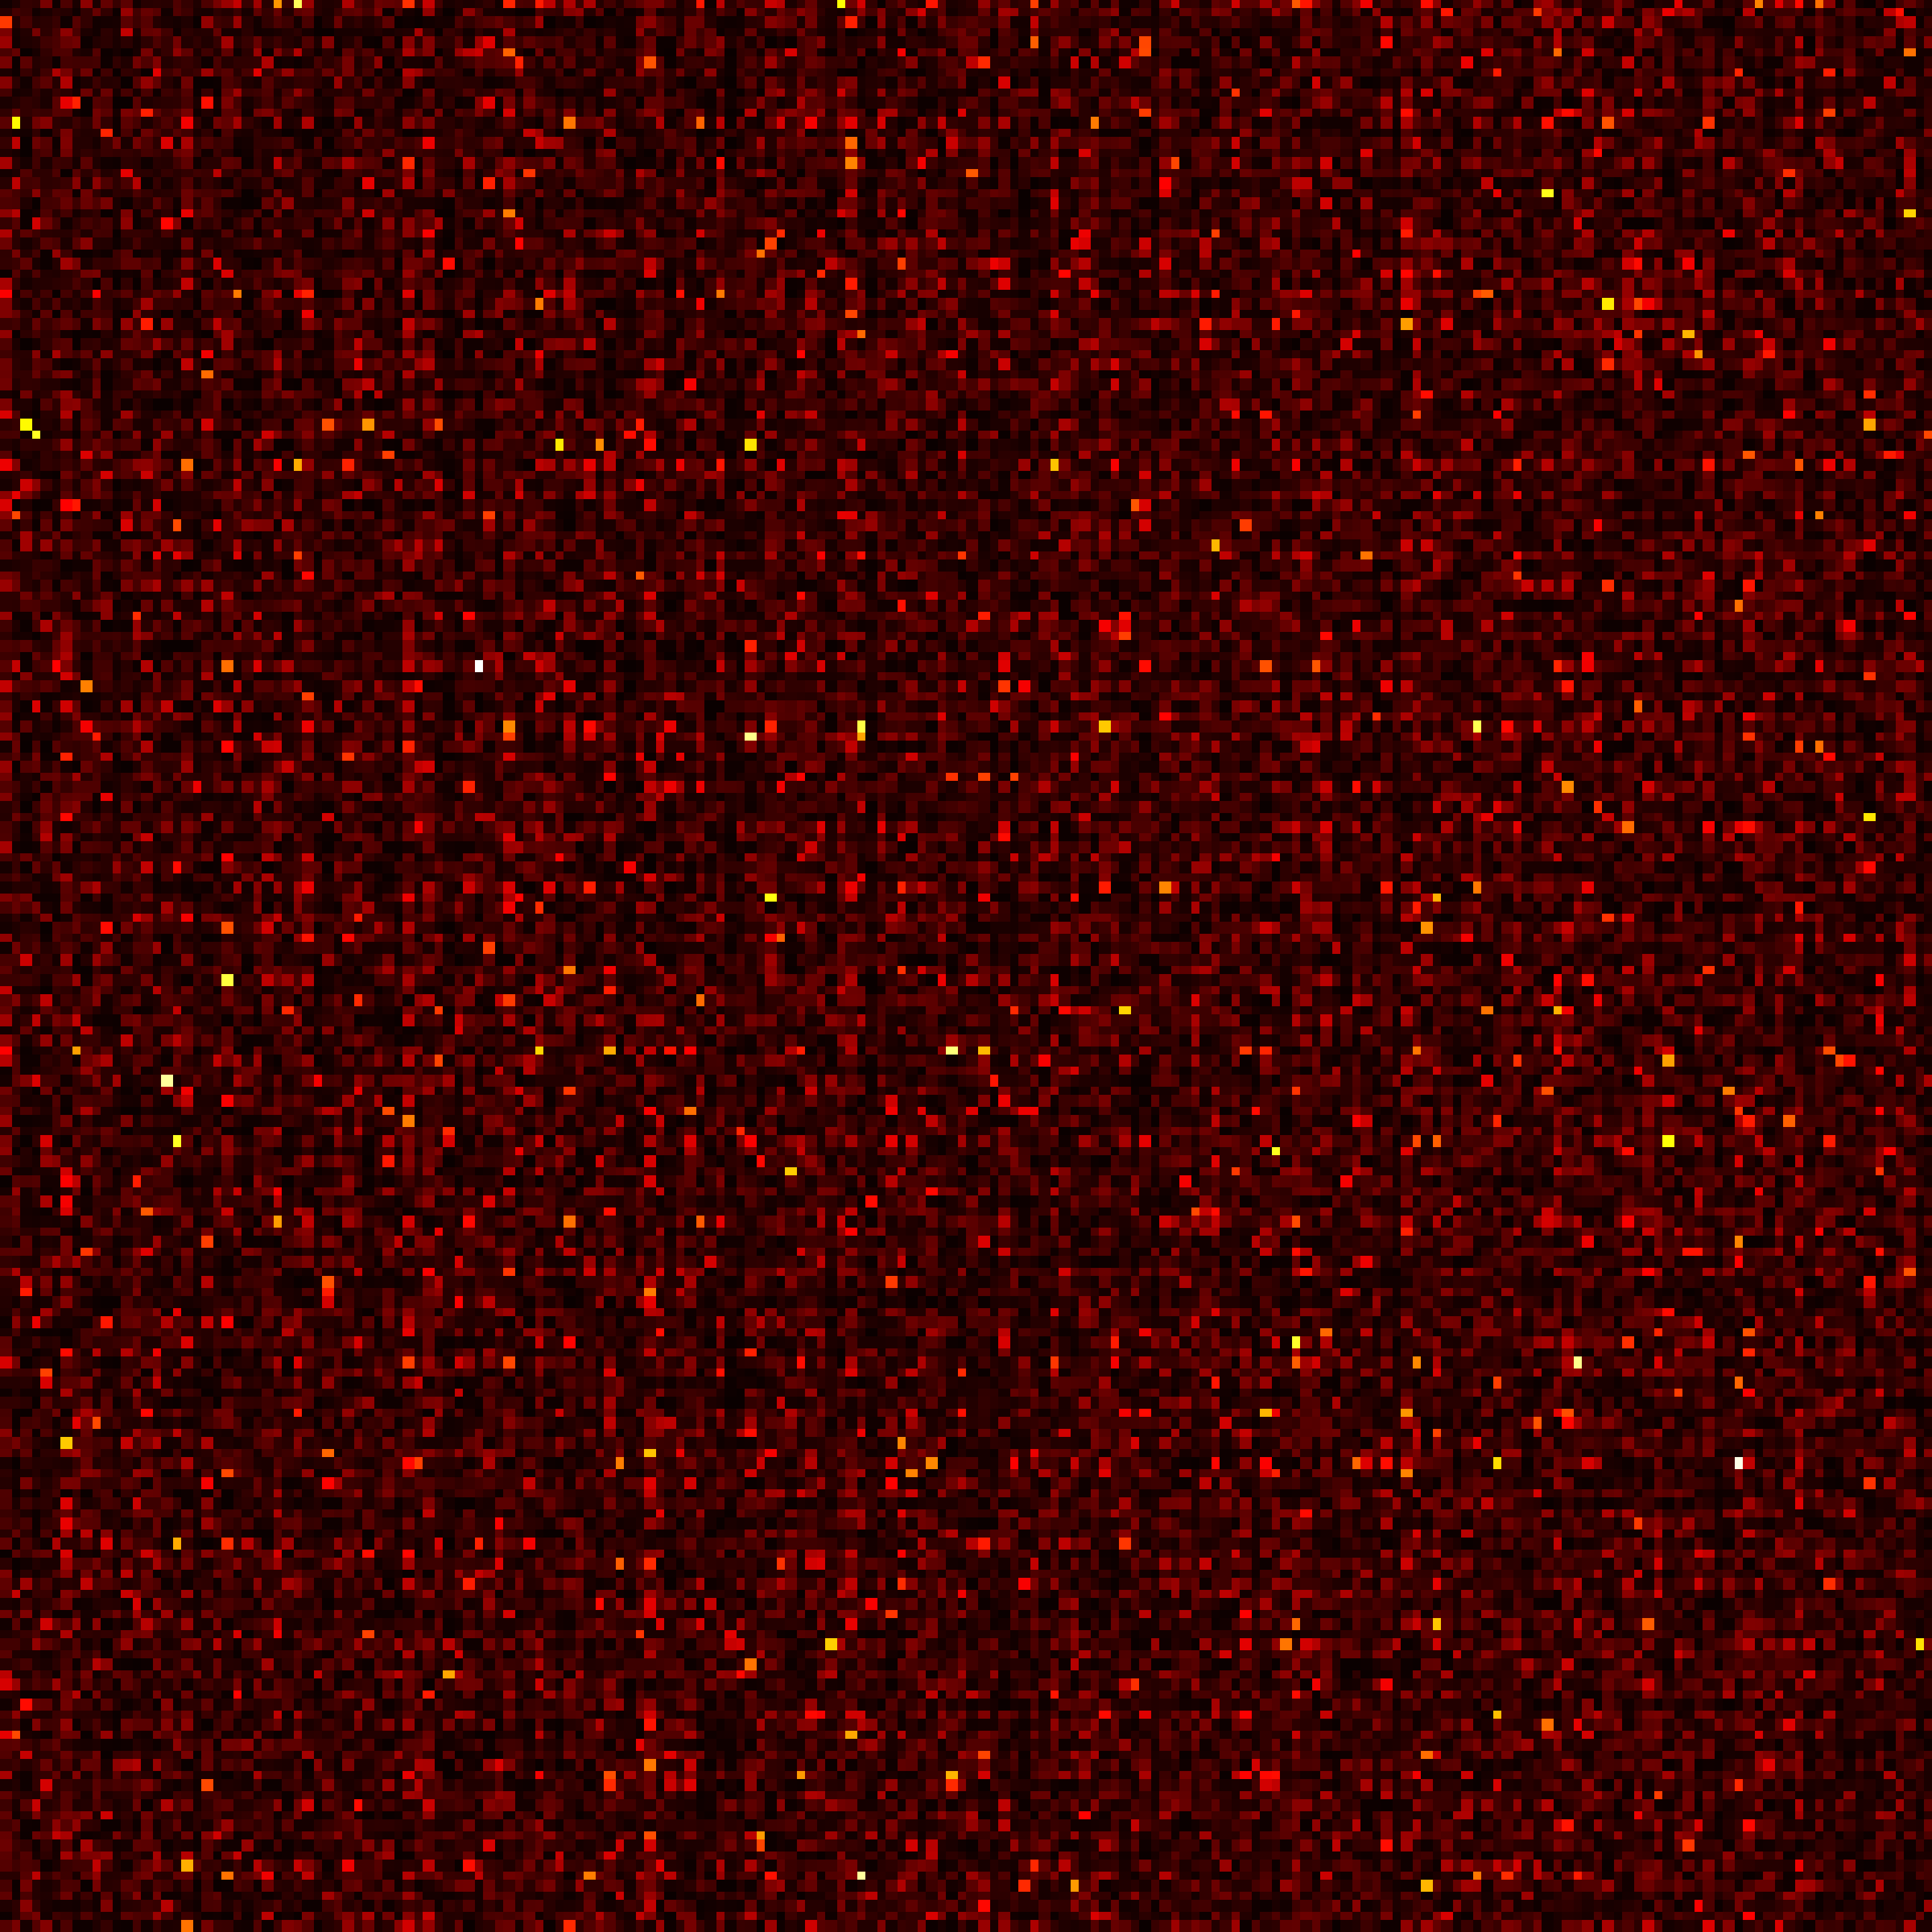
\includegraphics[width=\linewidth]{../Figs/Raster/msrc-cifar-nin-4pad-conv8-corr}}
    \caption{\textbf{Standard:} $g=1$}
    \label{fig:normalcovartest}
\end{subfigure}
~
\begin{subfigure}[b]{0.31\linewidth}
\centering
    \covarlabels{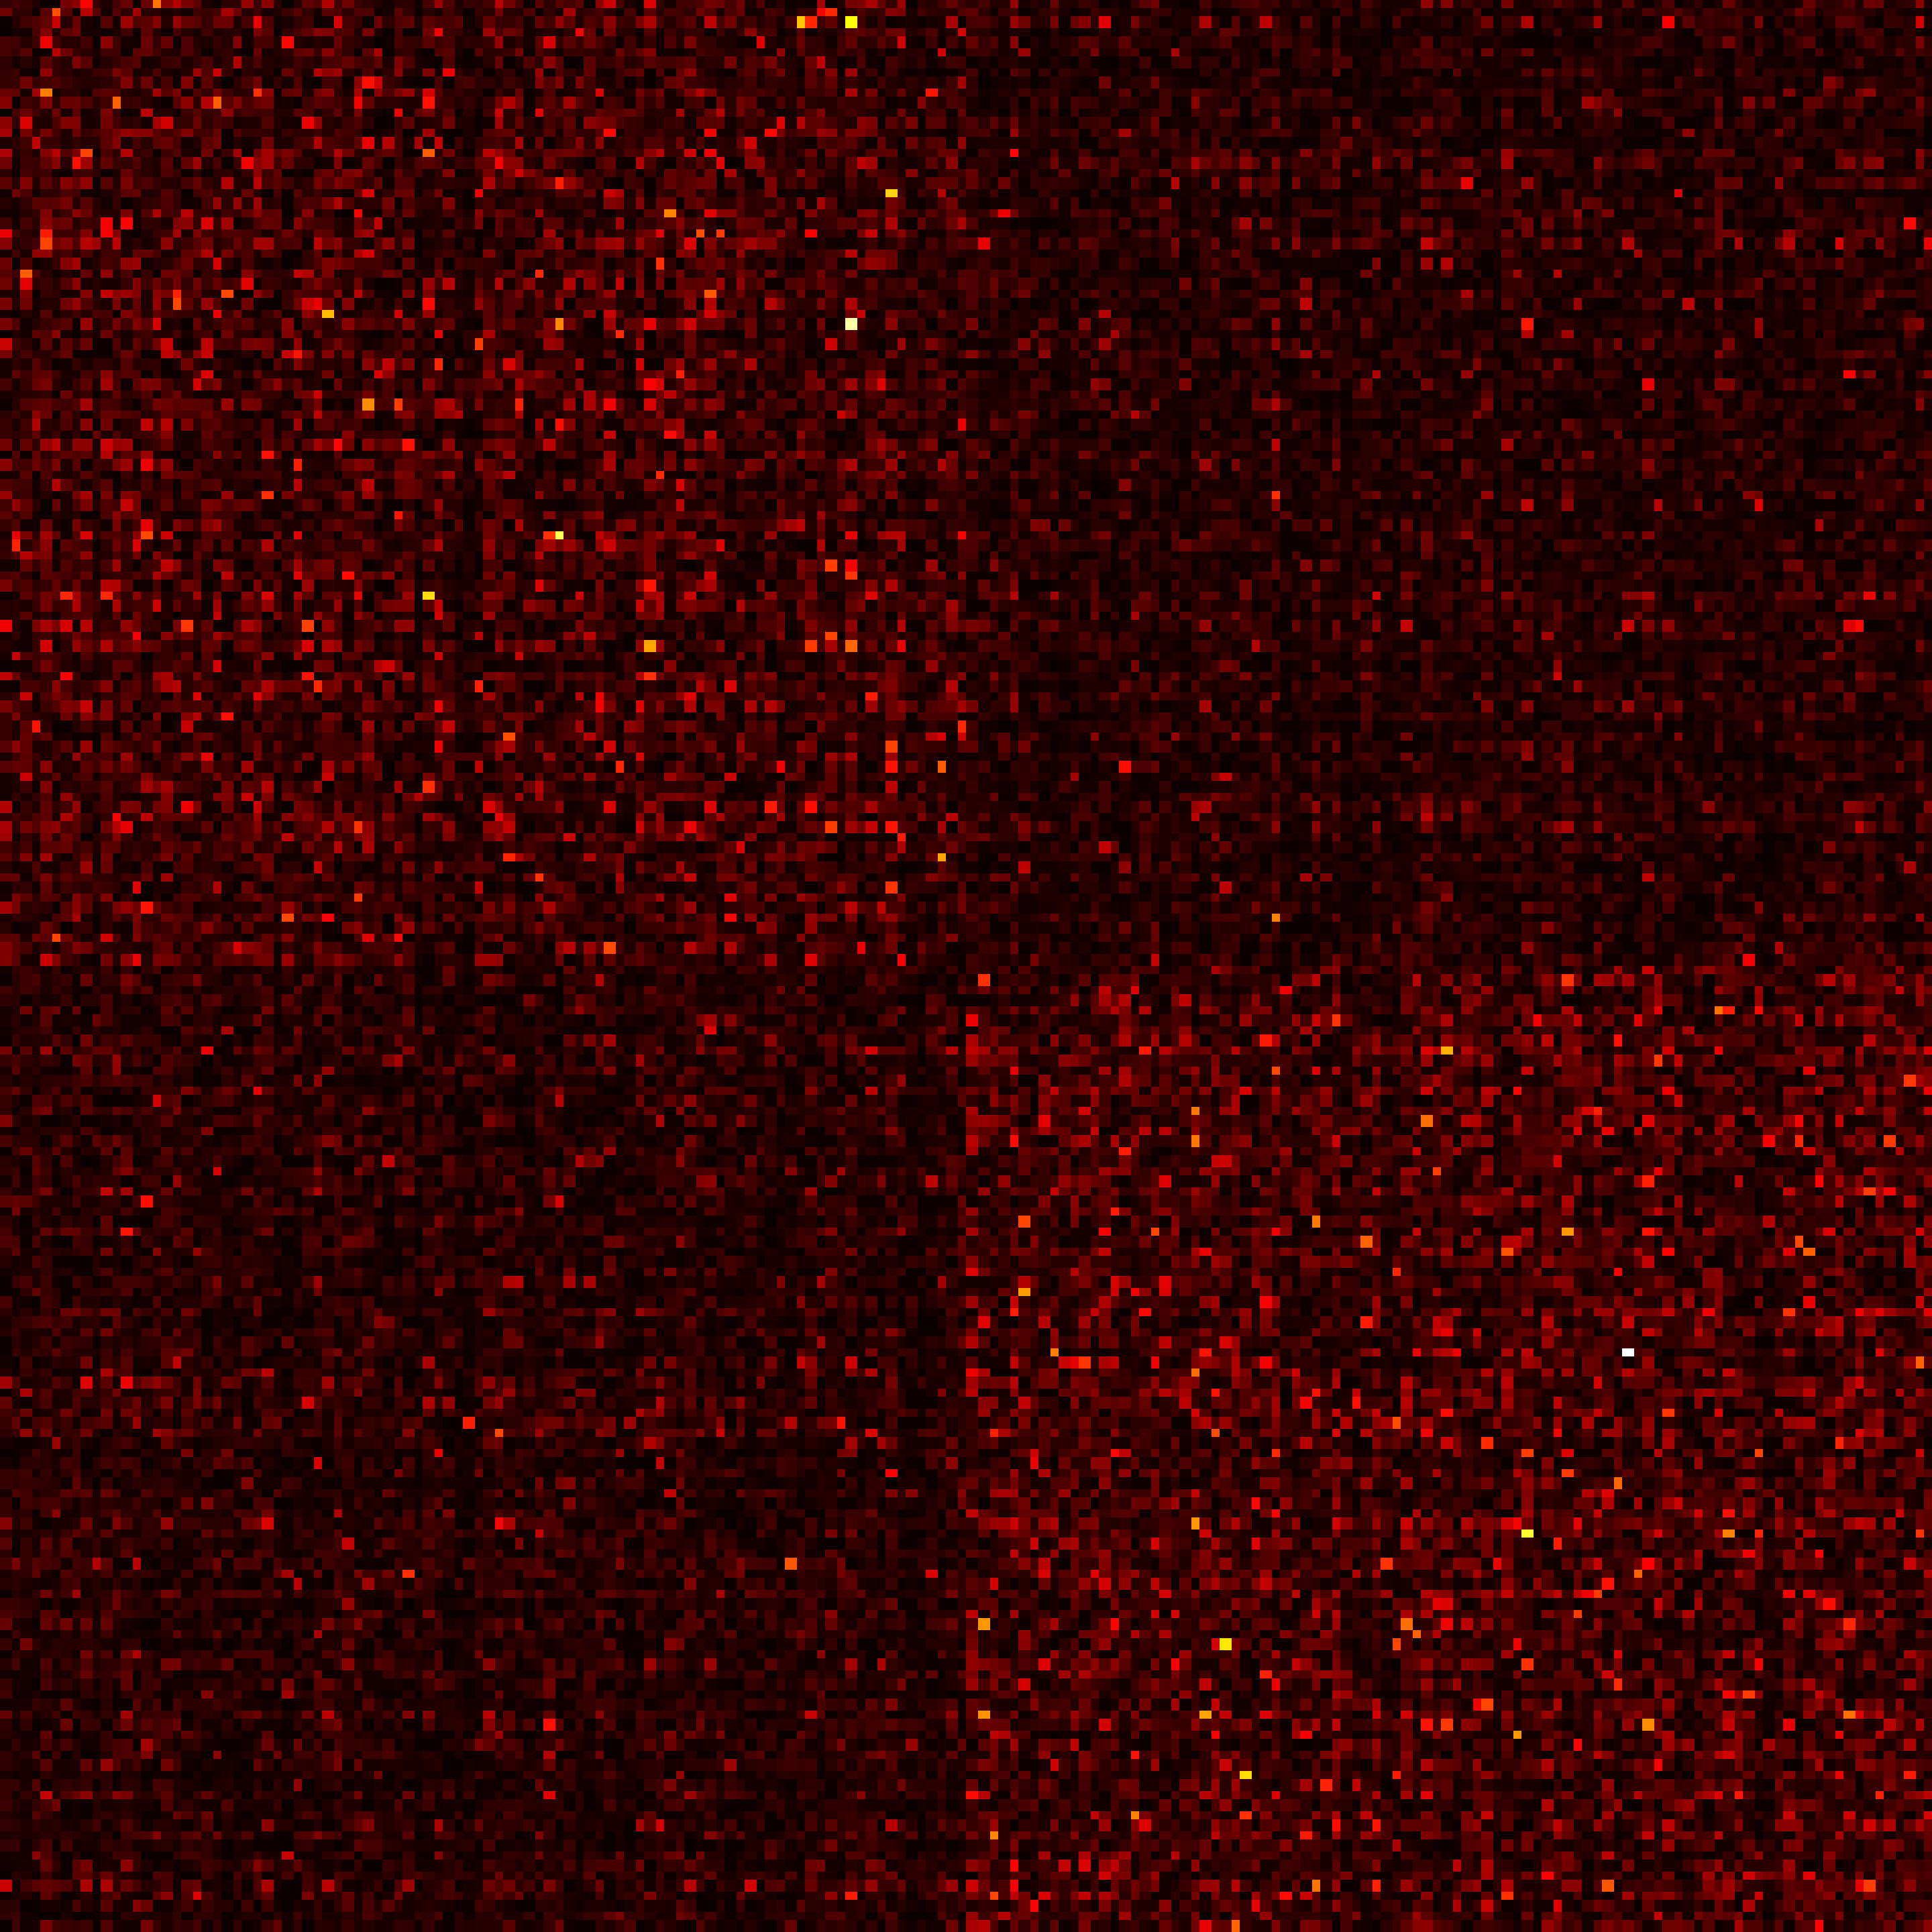
\includegraphics[width=\linewidth]{../Figs/Raster/msrc-cifar-nin-4pad-funnel4-convonly-conv8-corr}}
    \caption{\textbf{Root-4:} $g=2$}
    \label{fig:root4}
\end{subfigure}
%~
%\begin{subfigure}[b]{0.24\linewidth}
%\centering
%    \covarlabels{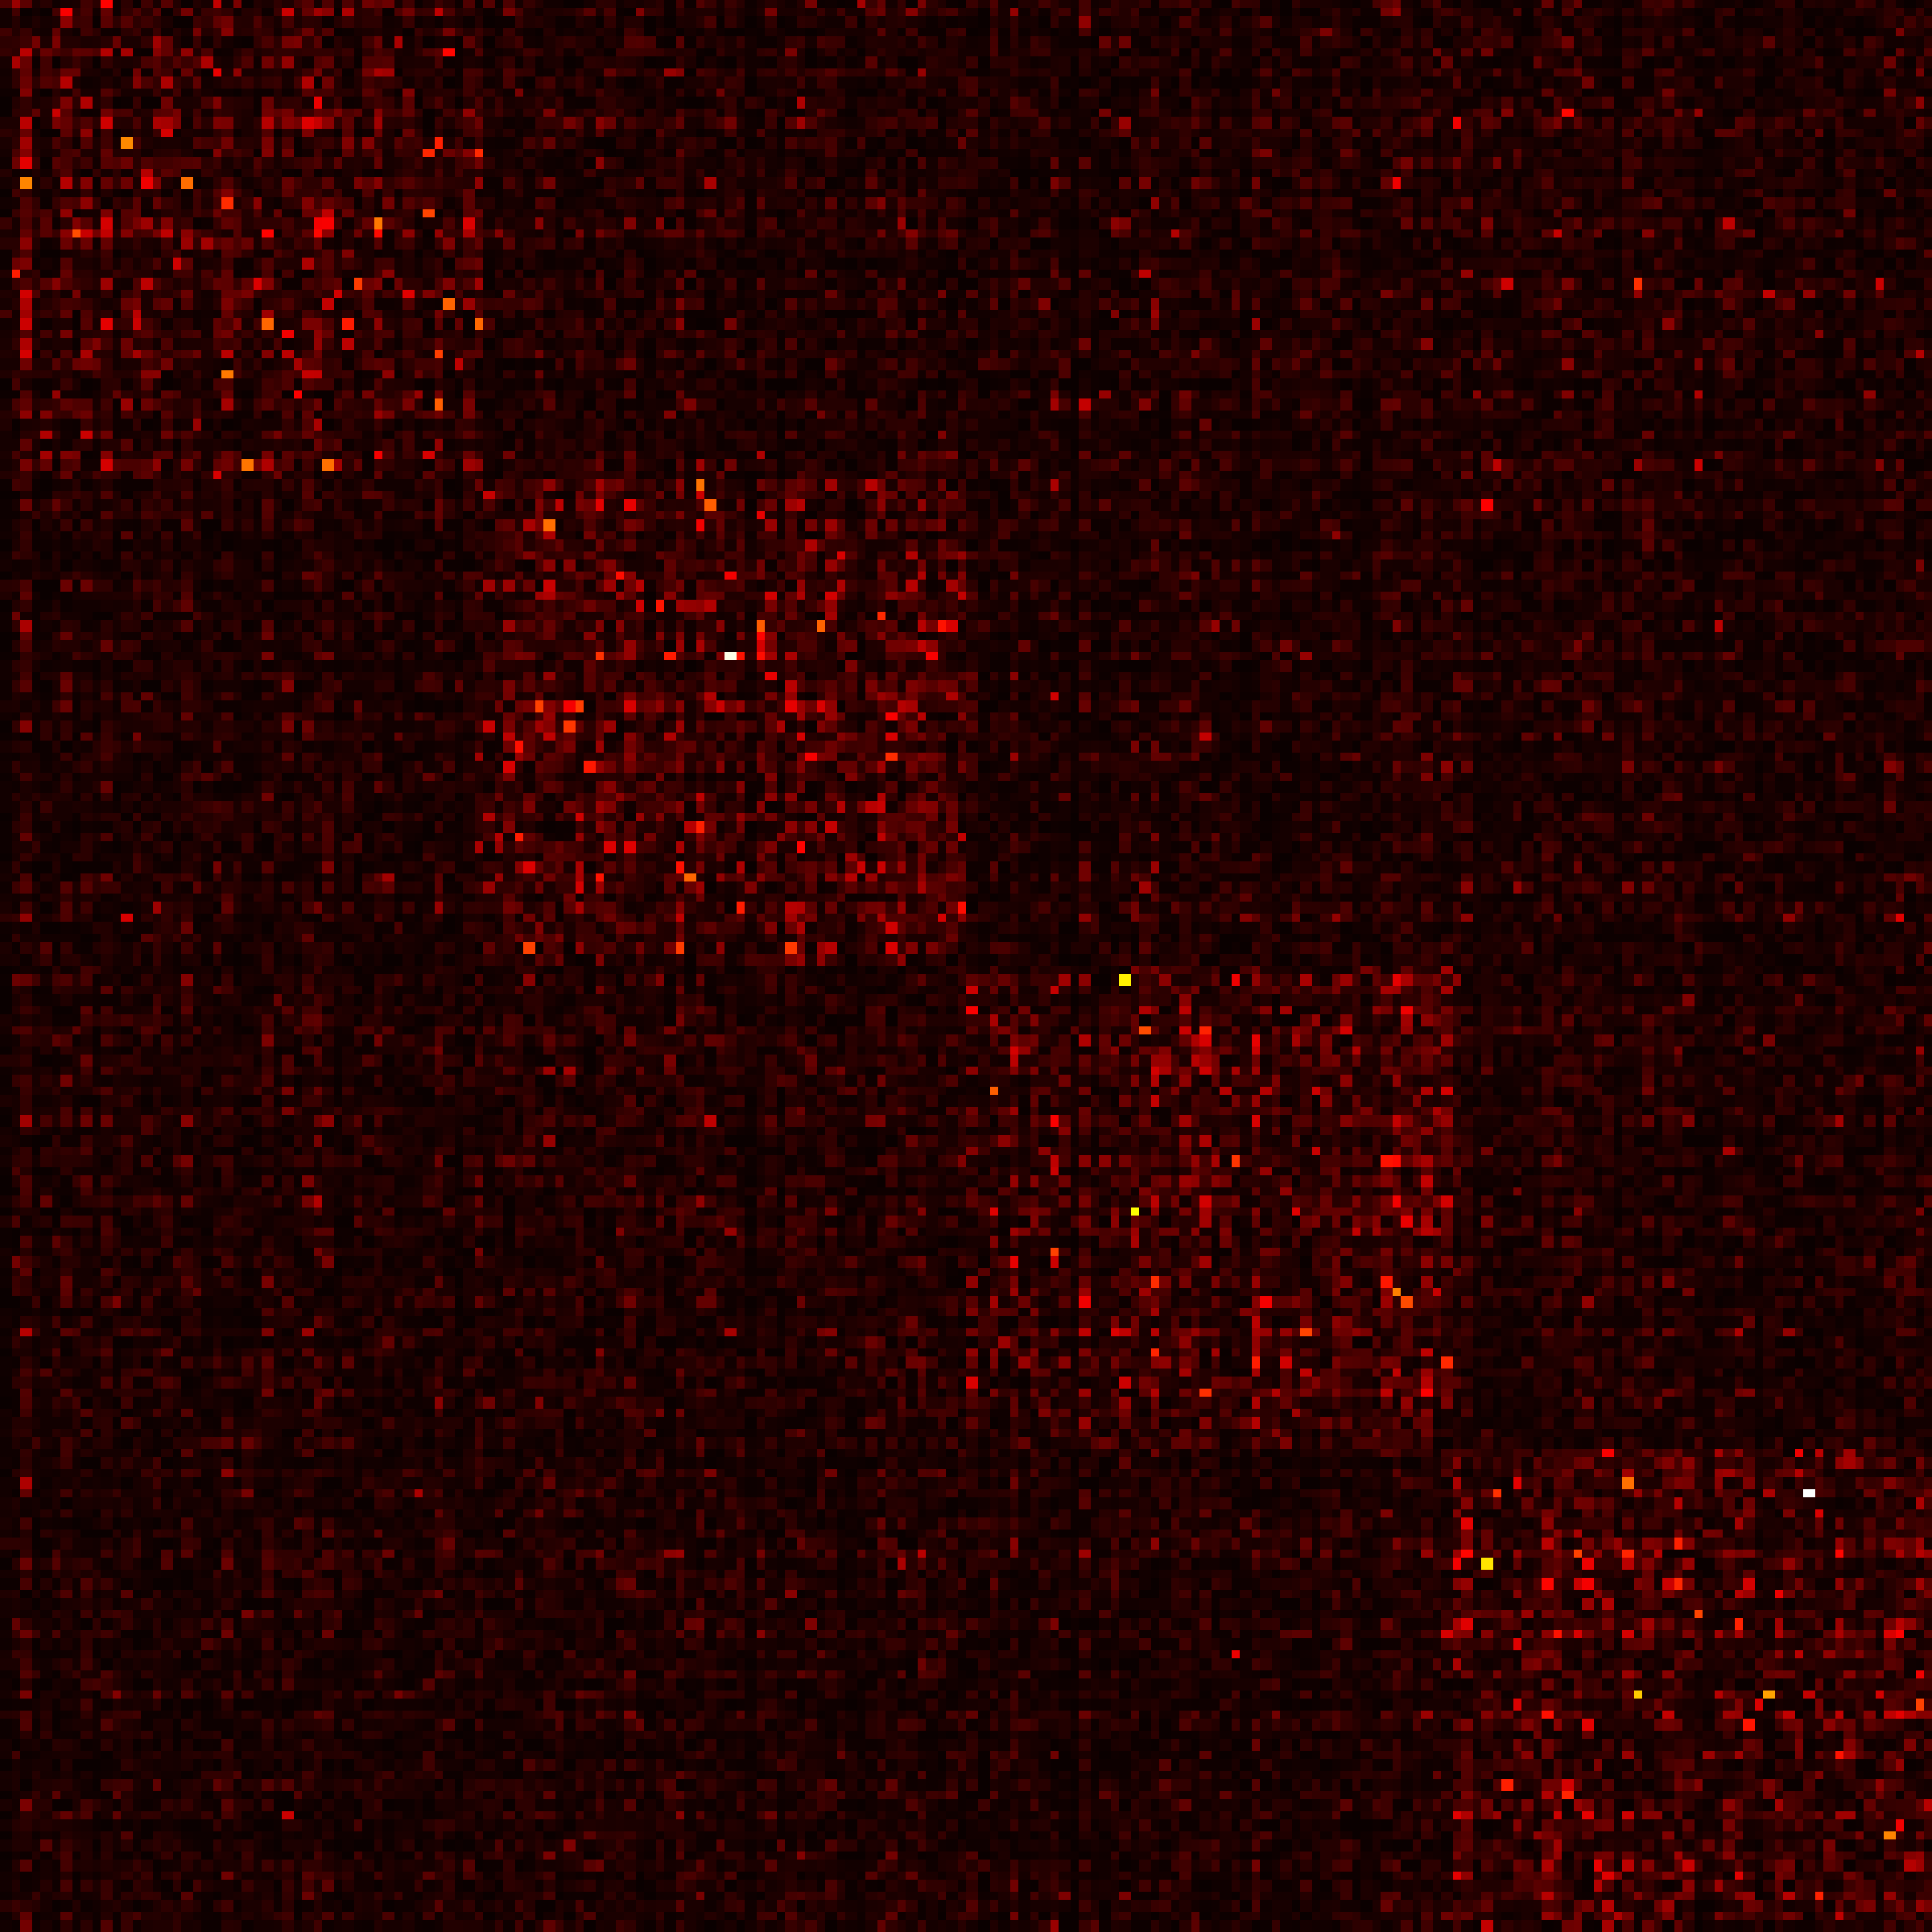
\includegraphics[width=\linewidth]{../Figs/Raster/msrc-cifar-nin-4pad-funnel8-convonly-conv8-corr}}
%    \caption{\textbf{Root-8:} 4 filter groups}
%    \label{fig:root8corr}
%\end{subfigure}
~
\begin{subfigure}[b]{0.31\linewidth}
\centering
    \covarlabels{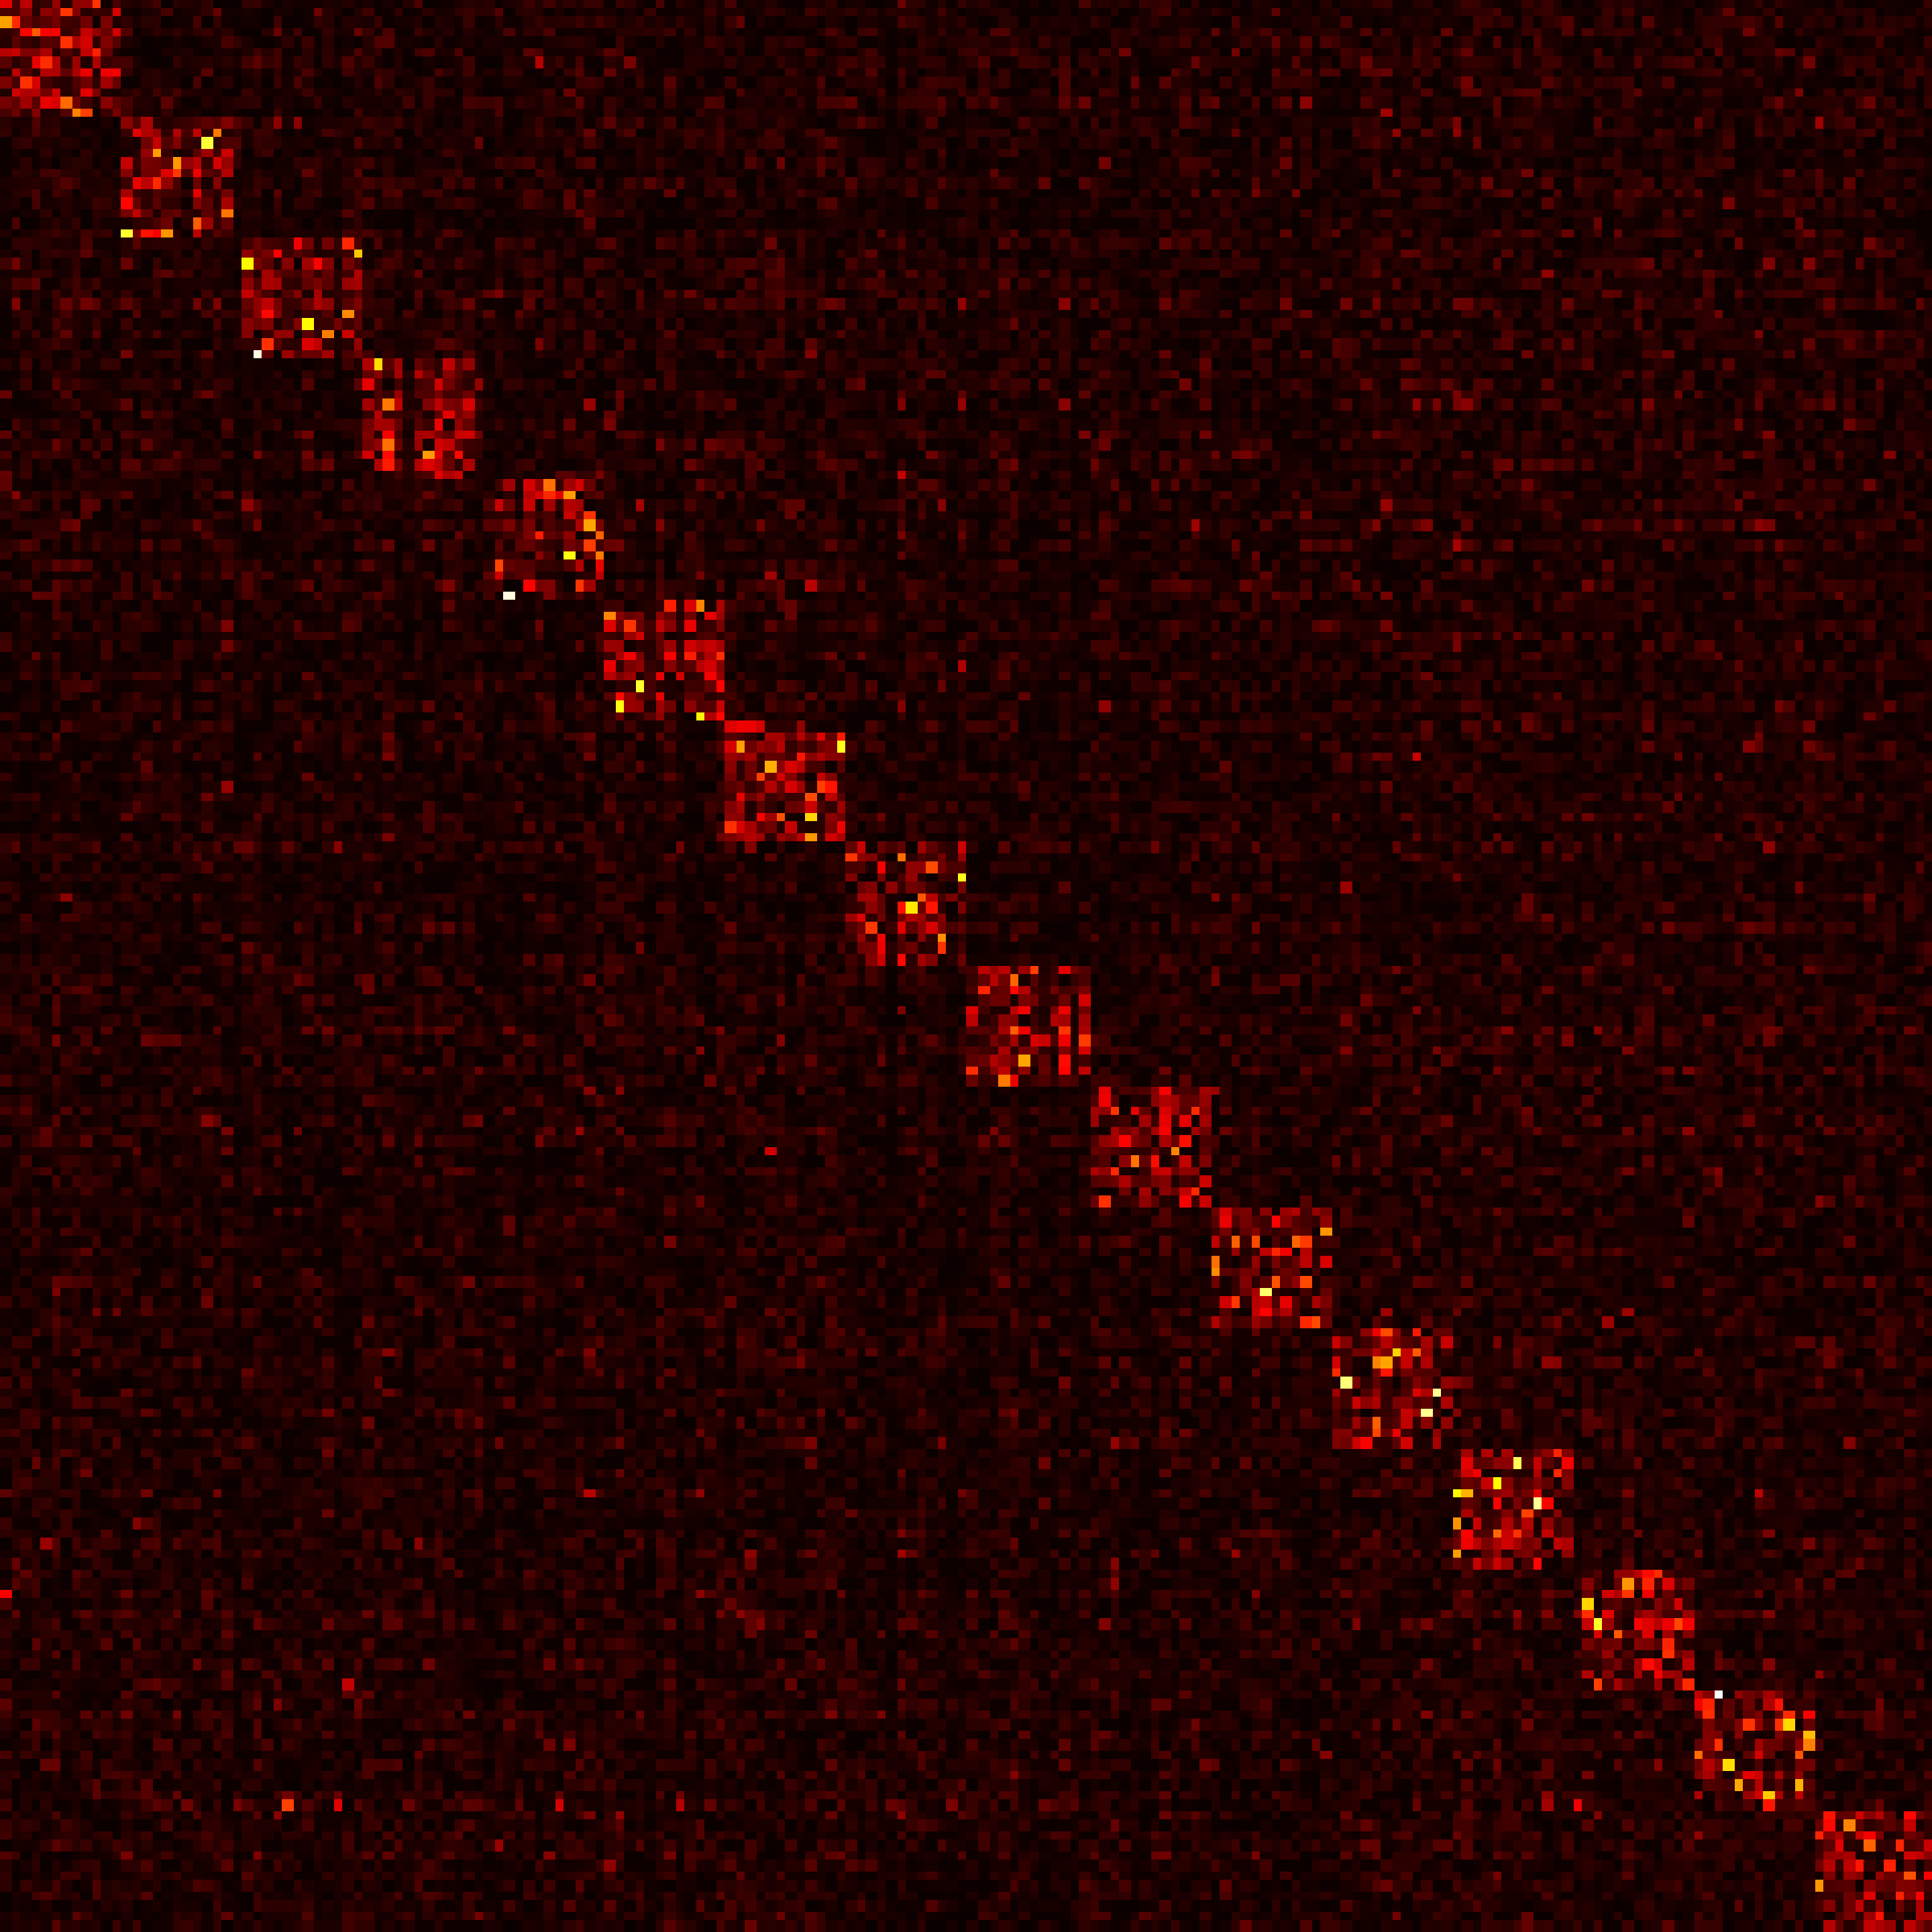
\includegraphics[width=\linewidth]{../Figs/Raster/msrc-cifar-nin-4pad-funnel32-convonly-conv8-corr}}
    \caption{\textbf{Root-32:} $g=16$}
    \label{fig:root32corr}
\end{subfigure}
\caption{The block-diagonal sparsity learned by a root-module is visible in the correlation of filters on layers \texttt{conv3a} and \texttt{conv2c} in the NiN network.}
\label{fig:covar}
\end{figure}
%Figure~\ref{fig:covar} shows the inter-layer correlation between the adjacent filter layers \texttt{conv2c} and \texttt{conv3a} in the network architectures outlined in Table~\ref{table:ninconfig} as evaluated on the CIFAR test set. The block-diagonalization enforced by the filter group structure (as illustrated in Fig.~\ref{fig:groupconfig}) is visible, more so with larger number of filter groups. This shows that the network learns an organization of filters such that the sparsely distributed strong filter relations, visible in \ref{fig:normalcovartest} as brighter pixels, are grouped into a denser block-diagonal structure, leaving a visibly darker, low-correlated background. See \S\ref{interlayercovar} for more images, and an explanation of their derivation.
\end{frame}

%%%%%%%%%%%%%%%%

\begin{frame}{Imagenet Results}

%We propose a new method for creating computationally efficient and compact convolutional neural networks (CNNs) using a novel sparse connection structure that resembles a tree root. This allows a significant reduction in computational cost and number of parameters compared to state-of-the-art deep CNNs, without compromising accuracy, by exploiting the sparsity of inter-layer filter dependencies. We validate our approach by using it to train more efficient variants of state-of-the-art CNN architectures, evaluated on the CIFAR10 and ILSVRC datasets. Our results show similar or higher accuracy than the baseline architectures with much less computation, as measured by CPU and GPU timings. For example, for ResNet 50, our model has 40% fewer parameters, 45% fewer floating point operations, and is 31% (12%) faster on a CPU (GPU). For the deeper ResNet 200 our model has 25% fewer floating point operations and 44% fewer parameters, while maintaining state-of-the-art accuracy. For GoogLeNet, our model has 7% fewer parameters and is 21% (16%) faster on a CPU (GPU).
Networks with root modules have similar or higher accuracy than the baseline architectures with much less computation.
\begin{itemize}
    \item ResNet 50\footnote{Caffe Re-implementation}: \textbf{40\%} smaller, \textbf{45\%} fewer FLOPS%, and is 31\% (12\%) faster on a CPU (GPU).
    \item ResNet 200\footnote{Based on Facebook Torch Model}: \textbf{44\%} smaller, \textbf{25\%} fewer FLOPS
    \item GoogLeNet: \textbf{7\%} smaller, \textbf{44\%} fewer FLOPS%, and is 21\% (16\%) faster on a CPU (GPU)
\end{itemize}
\vfill
But when you also \textbf{increase the number of filters}\ldots
\end{frame}

%%%%%%%%%%%%%%%%%%%%

\usebackgroundtemplate{
\tikz[overlay,remember picture] \node[opacity=0.5, at=(current page.center), yshift=-1cm] {
\centering
   \setlength{\fboxsep}{0pt}\setlength\fboxrule{0.5pt}\fbox{
   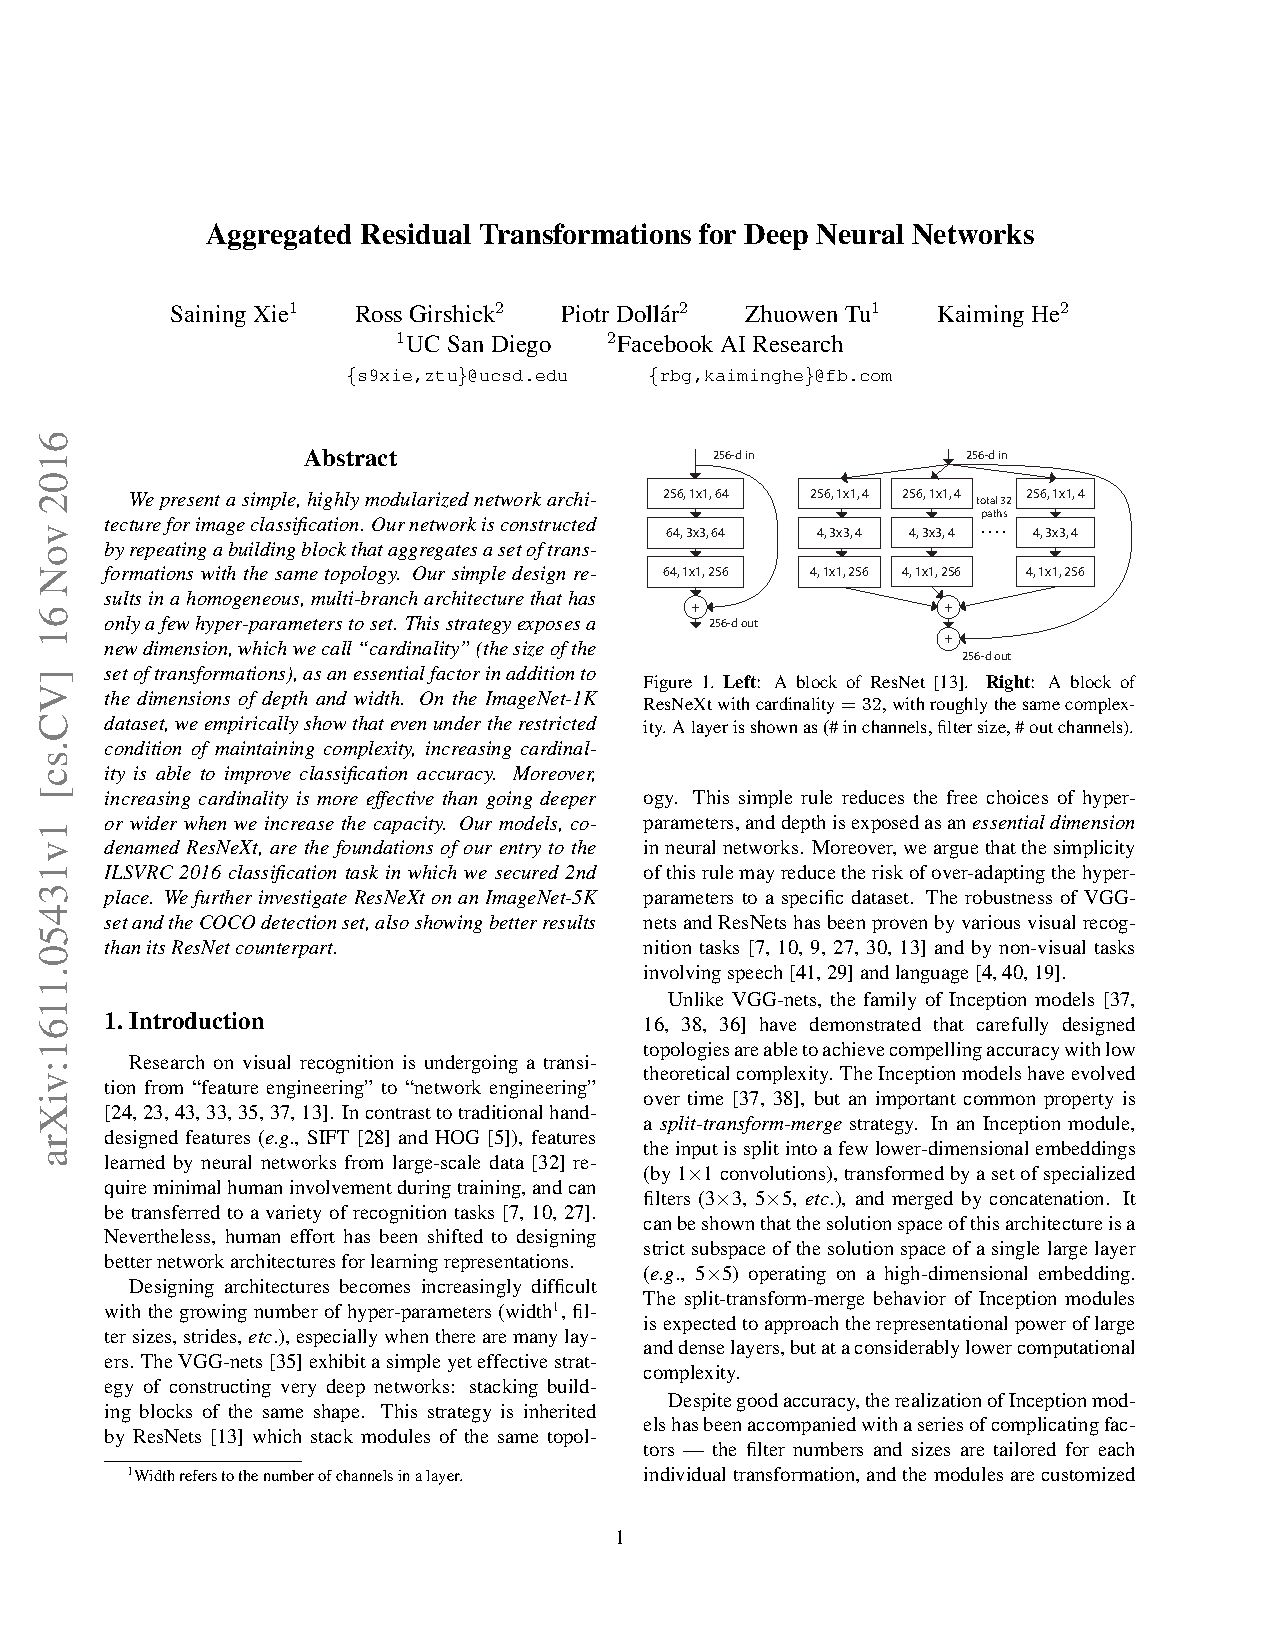
\includegraphics[width=0.9\paperwidth,page=1]{resnext.pdf}
   }
   };
}

\begin{frame}
\vfill
\centering
\colorbox{white}{
\setlength{\fboxsep}{0pt}\fbox{
\begin{minipage}{0.6\paperwidth}
   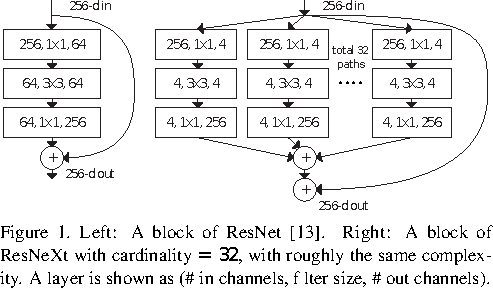
\includegraphics[width=0.6\paperwidth,page=1]{resnext-filterconfig.pdf}
   
   \begin{quote}
   \footnotesize
   ``Moreover, increasing cardinality is more effective than going deeper or wider when we increase the capacity.''
   \end{quote}
\end{minipage}
}
}
\end{frame}

\usebackgroundtemplate{}

%%%%%%%%%%%%%%%%%%%%
\section{Summary/Future Work}

%%%%%%%%%%%%%%%%%%%%
\begin{frame}{Summary}

  % Keep the summary *very short*.
  \begin{itemize}
	%\item Separable filter model show surprisingly high accuracy on what are considered challenging problems -- approx.\ 88\% top-5 accuracy on ILSVRC.
	\item Using structural priors:
	\begin{itemize}
    	\item Models are \textbf{less computationally complex}
	    \item They also use \textbf{less parameters}
	    \item They significantly help generalization in \textbf{deeper networks}
        \item They significantly help generalization with \textbf{larger datasets}
	\end{itemize}
	\item Are amenable to \textbf{model parallelization} (as with original AlexNet), for better parallelism across gpus/nodes
	%\item The restriction on what filter responses may be combined is an effective form of regularization, and helps prevent over-fitting.
  \end{itemize}
\end{frame}

%%%%%%%%%%%%%%%%%%%%
\begin{frame}{Future Work: Research}
    \begin{itemize}
        \item We don't always have enough knowledge of the domain to propose good structural priors
        \item Our results (and follow up work) do show however that current methods of training/regularization seem to have limited effectiveness in DNNs learning such priors themselves
        \item How can we otherwise learn structural priors?
    \end{itemize}
\end{frame}

\end{document}


